% ----------- Cover Master Thesis Faculty of Sciences ---------------
% This document should be compiled with pdflatex.  If you want to use
% latex to compile to dvi/ps, you have to convert the images to (e)ps
%                           -- December 2012
% -------------------------------------------------------------------
\RequirePackage{fix-cm}
\documentclass[12pt,a4paper]{book}

% ------------------------- Load packages ---------------------------
% You can eventually add these while you load other packages
% in case you want to integrate the titlepage with the rest of your thesis
% -------------------------------------------------------------------
\usepackage{graphicx,xcolor,textpos}
\usepackage{helvet}
\usepackage{listings}
\usepackage{csquotes}
\usepackage{amsmath}
\usepackage{amsfonts}
\usepackage{amssymb}
\usepackage{fancyhdr}


% ----------------------------- Headers  -----------------------------
\pagestyle{fancy}
\fancyhf{}
\fancyhead[RE]{\it\leftmark~ $\bigg|$ ~ \thepage}
\fancyhead[LO]{\it\thepage~ $\bigg|$ ~ \rightmark}
% \fancyfoot[C]{\thepage}
\renewcommand{\headrulewidth}{0pt}


% ----------------------- Chapters and Sections ----------------------
\usepackage{titlesec}
\titleformat{\chapter}{\normalfont\Huge}{}{24pt}{\Huge\it}
\titleformat{\section}{\normalfont\LARGE}{}{18pt}{\LARGE\it}



% ------------------------ Page settings -----------------------------
% If you change these, the cover layout will also change.  In that
% case you have to adjust the latter manually.
% --------------------------------------------------------------------

\topmargin -10mm
\textwidth 160truemm
\textheight 240truemm
\oddsidemargin 0mm
\evensidemargin 0mm

% ---------------------- textpos settings ----------------------------
% Some additional settings for the cover
% --------------------------------------------------------------------

\definecolor{green}{RGB}{172,196,0}
\definecolor{bluetitle}{RGB}{29,141,176}
\definecolor{blueaff}{RGB}{0,0,128}
\definecolor{blueline}{RGB}{82,189,236}
\setlength{\TPHorizModule}{1mm}
\setlength{\TPVertModule}{1mm}



% --------------------- Code Formatting ------------------------------
\definecolor{mygreen}{rgb}{0,0.6,0}
\definecolor{mygray}{rgb}{0.5,0.5,0.5}
\definecolor{mymauve}{rgb}{0.58,0,0.82}

\lstset{ %
  backgroundcolor=\color{white},   % choose the background color; you must add \usepackage{color} or \usepackage{xcolor}
  basicstyle=\footnotesize\ttfamily,% the size of the fonts that are used for the code
  breakatwhitespace=false,         % sets if automatic breaks should only happen at whitespace
  breaklines=true,                 % sets automatic line breaking
  captionpos=b,                    % sets the caption-position to bottom
  commentstyle=\color{mygreen},    % comment style
  deletekeywords={...},            % if you want to delete keywords from the given language
  escapeinside={\%*}{*)},          % if you want to add LaTeX within your code
  extendedchars=true,              % lets you use non-ASCII characters; for 8-bits encodings only, does not work with UTF-8
  frame=single,                    % adds a frame around the code
  keepspaces=true,                 % keeps spaces in text, useful for keeping indentation of code (possibly needs columns=flexible)
  keywordstyle=\color{blue},       % keyword style
  language=C++,                 % the language of the code
  otherkeywords={*,...},           % if you want to add more keywords to the set
  numbers=left,                    % where to put the line-numbers; possible values are (none, left, right)
  numbersep=5pt,                   % how far the line-numbers are from the code
  numberstyle=\tiny\color{mygray}, % the style that is used for the line-numbers
  rulecolor=\color{black},         % if not set, the frame-color may be changed on line-breaks within not-black text (e.g. comments (green here))
  showspaces=false,                % show spaces everywhere adding particular underscores; it overrides 'showstringspaces'
  showstringspaces=false,          % underline spaces within strings only
  showtabs=false,                  % show tabs within strings adding particular underscores
  stepnumber=1,                    % the step between two line-numbers. If it's 1, each line will be numbered
  stringstyle=\color{mymauve},     % string literal style
  tabsize=2,                     % sets default tabsize to 2 spaces
  title=\lstname                   % show the filename of files included with \lstinputlisting; also try caption instead of title
}




\begin{document}

% ----------------------- Cover --------------------------------------
% Please fill in:
% - The title and subtitle (if applicable)
%         to include a formula in the title or subtitle
%         use  \form{$...$}
% - Your name
% - Your (co)supervisor, mentor (if applicable)
% - Your master
% - The academic year
% --------------------------------------------------------------------
\thispagestyle{empty}
\newcommand{\form}[1]{\scalebox{1.087}{\boldmath{#1}}}
\sffamily
%
\begin{textblock}{191}(-24,-11)
\colorbox{green}{\hspace{139mm}\ \parbox[c][18truemm]{52mm}{\textcolor{white}{Faculty of Science \\ LStat}}}
\end{textblock}
%
\begin{textblock}{70}(-18,-19)
\textblockcolour{}
\includegraphics*[height=19.8truemm]{img/LogoKULeuven}
\end{textblock}
%
\begin{textblock}{160}(-6,63)
\textblockcolour{}
\vspace{-\parskip}
\flushleft
\fontsize{40}{42}\selectfont \textcolor{bluetitle}{Predictive Maintenance}\\[1.5mm]
\fontsize{20}{22}\selectfont In Informationally Sparse Systems
\end{textblock}
%
%\begin{textblock}{82}(50,103)
%\textblockcolour{}
%\vspace{-\parskip}
%\flushleft
%\fbox{\parbox{79mm}{The background can be left blank or you can insert an image (maximum height 10 cm, width variable, mind author’s rights…). NO logos (you can use the logos inside the manuscript, but not on front or back cover). \textit{Delete this textbox.}}}
%\end{textblock}
%
\begin{textblock}{160}(8,153)
\textblockcolour{}
\vspace{-\parskip}
\flushright
\fontsize{14}{16}\selectfont \textbf{Richard PODKOLINSKI}
\end{textblock}
%
\begin{textblock}{70}(-6,191)
\textblockcolour{}
\vspace{-\parskip}
\flushleft
Supervisor: Prof.~dr.Luc De Raedt\\[4.5pt]
%\textcolor{blueaff}{Affiliation \textsl{(optional)}}\\[5pt]
Co-supervisor: Wannes Meert\\[4.5pt]
%\textcolor{blueaff}{Affiliation \textsl{(optional)}}\\[5pt]
%Mentor: \textsl{(optional)}\\[-2pt]
%\textcolor{blueaff}{Affiliation \textsl{(optional)}}\\
\end{textblock}
%
\begin{textblock}{160}(8,191)
\textblockcolour{}
\vspace{-\parskip}
\flushright
Thesis presented in\\[4.5pt]
fulfillment of the requirements\\[4.5pt]
for the degree of Master of Science\\[4.5pt]
in Statistics\\
\end{textblock}
%
\begin{textblock}{160}(8,232)
\textblockcolour{}
\vspace{-\parskip}
\flushright
Academic year 2015-2016
\end{textblock}
%
\begin{textblock}{191}(-24,248)
{\color{blueline}\rule{550pt}{5.5pt}}
\end{textblock}
%
\vfill
\newpage
\thispagestyle{empty}

\pagenumbering{gobble}
\vspace*{570px}

\scriptsize\sffamily{\setlength{\parindent}{0ex}\copyright{}~2016~KU Leuven -- Faculty of Science, Richard Podkolinski, Leuven Statistics Research Centre (LStat), Celestijnenlaan 200 B, bus 5307, 3001 Heverlee, Belgium.}

\bigskip
\scriptsize\sffamily{\setlength{\parindent}{0ex}Without written permission of the promotors and the authors it is forbidden to reproduce or adapt in any form or by any means any part of this publication. Requests for obtaining the right to reproduce or utilize parts of this publication should be addressed to KU Leuven, Faculteit Wetenschappen, Geel Huis, Kasteelpark Arenberg 11 bus 2100, 3001 Leuven (Heverlee), Telephone +32 16 32 14 01.}
\bigskip

\scriptsize\sffamily{\setlength{\parindent}{0ex}A written permission of the promotor is also required to use the methods, products, schematics and programs described in this work for industrial or commercial use, and for submitting this publication in scientific contests.}


\newpage


% In case you want to integrate the TeX-file for the titlepage
% with the rest of your thesis, you cab continue below
% ------------------------- First pages ---------------------------
% For table of contents, acknowlegments, ...
% -----------------------------------------------------------------
\normalsize
\rmfamily
\setcounter{page}{0}
\pagenumbering{roman}


\thispagestyle{empty}
\vspace*{20px}
\begin{displayquote}
"I conceive the mind as a moving thing, and arguments as motive forces driving it in one direction or the other" 
\end{displayquote}

\begin{flushright}
\textit{John Craig}
\end{flushright}

\vspace*{25px}

\section*{Acknowledgments}

No man is an island.

While a single name appears on the cover of this document, it should not be implied that anything was, or could be done, alone. Everyone is the product of their environments and I've had the esteemed privilege to be assisted and inspired by many wonderful people. 

So my great appreciation to Ewa Podkolinska, Jerzy Podkolinski, Alina Kroeker, Raymond Kroeker, Tom Ruette, Wannes Meert, Mathias Verbeke, Gregory Schiano, Jan Aerts, Gerda Claeskens, Luc De Raedt, Roel Braekers, Geert Verbeke, Eric Schmitt, Rui Barbosa, Stijn Van Weezel, Akshat Dwivedi, Irzam Hardiansyah, Zhu Meng, Sytze Elzinga, Justin Fischedick and most importantly Rianne Hartemink.

Thank you for your support and motivation. 

\begin{flushright}
\textit{Richard Podkolinski}
\\
2016 
\\
Den Haag
\\
The Netherlands
\end{flushright}

\vspace*{25px}

\section*{Intended Audience}

Good research is the kind that is capable of taking a complex topic making it accessible to a broader audience. In an effort to adhere to that standard, the intended audience of this thesis is not a pure mathematician, rather a general practitioner in the area of predictive maintenance or reliability analysis. Emphasized is the development of understanding and intuition for the underlying models and how to handle edge cases. 

While great effort is undertaken to be as accessible as possible, a certain degree of mathematical development is required to understand this text. Recommended is an understanding of the calculus of probabilities at the level of Blitzstein and Huang\cite{Blitzstein2014} as well as a first course on Bayesian linear models at the level of McElreath\cite{McElreath2016}. A basic understanding of how basic linear models are fit and their performance evaluated is required.

To ensure access to rigorous results, an extensive list of references and resources are made available at the end of each chapter, dubbed "Extended Reading". These resources elucidate many of the technical aspects of the modeling process and mathematical foundations which are beyond the scope of this text.

\newpage

\section*{Abstract}


The evolution of predictive maintenance strategies is not universally applicable in all domains. The increased ability of organizations to capture a wider breadth and greater volume of data has lead to a narrow research focus that cannot be easily translated to all domains. Industrial-scale solar power is one of these domains, which has limited access to condition monitoring data. Yet, the need in the domain for predictive maintenance is greater than ever.

This thesis addresses the development of a predictive maintenance process in informationally sparse systems, specifically using the photovoltaic inverters as the object of interest. It seeks to fill the void in the current literature on predictive maintenance in environments where there is limited access to operational data. It addresses the problem through the use of Bayesian time-to-event analysis, a statistical modeling approach used to estimate the remaining lifetime of an object. As such, it progresses through the process of developing a predictive maintenance system starting from the mathematics of time-to-event analysis through to the practical concerns of deploying an process. Finally, it presents an application using simulated data using Stan, the probabilistic programming language.


\newpage

\section*{List of Abbreviations}

\begin{itemize}

\item[] PV -  Photovoltaic
\item[] BOS - Balance of Systems
\item[] AC - Alternating Current
\item[] DC - Direct Current
\item[] kWh - KiloWatt Hours

\item[] pdf - Probability Density Function
\item[] cdf - Cumulative Distribution Function
\item[] MLE - Maximum Likelihood Estimation
\item[] MCMC - Markov Chain Monte Carlo
\item[] HMC - Hamiltonian Monte Carlo

\item[] C-Index - Concordance Index
\item[] WAIC - Widely Applicable Information Criterion
\item[] DIC - Deviance Information Criterion

\item[] MSE - Mean-Squared Error
\item[] MAE - Mean-Absolute Error

\item[] AUC - Area Under Curve
\item[] ROC - Receiver Operating Conditions


\end{itemize}

\newpage

\section*{List of Symbols}

\begin{itemize}

\item[] $T$ - Random variable for a lifetime
\item[] $t$ - Realization of the above random variable; an instance of time.
\item[] $Y$ - Random variable for observed lifetimes
\item[] $y$ - Realization of the above random variable; an observed instance of time.
\item[] $d$ - Censoring Indicator
\item[] $\theta$ - Vector of Unknown Parameters
\item[] $\theta^s$ - Vector of Parameters from Completed Simulations
\item[] $\Gamma(\cdot)$ - The Gamma Function
\item[] $f(\cdot)$ - Probability Density Function
\item[] $F(\cdot)$ - Cumulative Distribution Function
\item[] $S(\cdot)$ - Survival Function (Reliability Function)
\item[] $h(\cdot)$ - Hazard Function (Conditional Failure Rate, Intensity, Force of Mortality)
\item[] $H(\cdot)$ - Cumulative Hazard Function
\item[] $h_0(\cdot)$ - Baseline Hazard Function
\item[] $H_0(\cdot)$ - Baseline Cumulative Hazard Function
\item[] $I(\cdot)$ - Indicator Function
\item[] $|\cdot|$ - Cardinality of a Set
\item[] $g(\cdot)$ - Undefined Lifetime Offset Function
\item[] $\mathfrak{g}(\cdot)$ - Undefined Frailty Distribution

\item[] $\mathbb{P}_c$ - Probability of Concordance
\item[] $\mathbb{P}_d$ - Probability of Discordance

\item[] $\mathcal{G}$ - A Graph
\item[] $\mathcal{V}$ - Set of Graph Vertices 
\item[] $\mathcal{E}$ - Set of Graph Edges 

\item[] $\text{elpd}$ - Expected Log Pointwise Predictive Density for a New Dataset
\item[] $\text{lpd}$ - Log Pointwise Predictive Density
\item[] $\hat{p}$ - Effective Number of Parameters

\end{itemize}



\tableofcontents
\thispagestyle{empty}



\clearpage\thispagestyle{empty}\null\newpage
% -------------------------- Proper text --------------------------
% Introduction, chapters, ...
% -----------------------------------------------------------------
\setcounter{page}{0}
\pagenumbering{arabic}


\chapter*{Introduction}
\markboth{Introduction}{Introduction}
\addcontentsline{toc}{chapter}{Introduction}
\thispagestyle{empty}


Maintenance is not sexy, but it is essential. It is the immune system of the modern industrialized world. Without it, the myriad of systems we depend on for safeguarding our collectively quality of life would rapidly deteriorate and disappear. Yet, few sing the praises of the multitude of technicians and engineers which are responsible for ensuring trains run on time, computer systems remain accessible or that bridges do not suddenly collapse. Paradoxically, this lack of visibility is a testament to the uninterrupted success of these activities. 

The preceding decades have brought with them rapid innovation in the area of maintenance. What has historically been a manual and labor-intensive activity is increasingly becoming a scientific process, one that leverages technology to optimize operations. Modernization has meant going beyond traditional methods of maintenance based on scheduled inspection or reactivity and moving towards those that utilize data and act before failure occurs. Such a trend can have a widespread impact on operational expenses. Reactive methods generally incur greater costs due to downtime and the need for more expensive replacement parts. Scheduled inspections share similar pitfalls, requiring downtime, specialized machinery and also running the risk of inadvertent damage to the objects they seek to maintain. Predictive maintenance minimizes many of these drawbacks. Judgments about the state of a device are made as a result of continuous monitoring of actual operating conditions\cite{Mobley2002}. This reduces downtime and allows for a better allocation of maintenance resources. Most importantly, predictive maintenance enables faults to be detected \textit{before} failure allowing for contingencies, such as repair or replacement, to ensure constant output.


The evolution of predictive maintenance owes much to the continued development of sensor technology. More reliable, accurate, and most importantly, inexpensive sensors have enabled continuous monitoring in a wider range of domains. Many modern devices come with built-in sensors that record output or other context-specific data that can be used to assess health. Increasingly, many also include connectivity that allows telemetry to be retrieved remotely and on demand. This reality is likely what has spurred widespread innovation in the field, with more than half of the publications on predictive maintenance emerging within the last decade.\footnote{Based on Search: Limo = 703 / 989 and Google Scholar = 3300 / 5450} Unfortunately, this data gluttony has also led to a form of tunnel vision, with the majority of this work dedicated to enabling predictive maintenance exclusively in informationally rich contexts. As a result, authors are predominantly preoccupied with domains where data is high dimensional, time-dependent, with fine granularity and encoded without error. 


While the future may make these ideal circumstances ubiquitous, there is still a wide set of domains where this is not a reality. Sensors may have become increasingly cheap and plentiful but they can still be expensive in relative terms. The majority of the sensors included in new products are meant to extend functionality and the continuous monitoring they enable is an fortunate but inadvertent consequence. Yet, for many devices the inclusion of additional sensors means an increase in manufacturing costs, which is often prohibitive. No product developer of sound mind would argue for the inclusion of a sensors in a t-shirt to prevent stitching failure. The sensors would vastly increase the final cost of the original product. However, this kind of cost-benefit dilemma is found throughout numerous domains where the sensor costs are high relative to the manufacturing cost of the product. In these domains, data is rarely high dimensional, time-dependent, fine and encoded without error. Despite these limitations, there is still a need for predictive maintenance. 

This thesis will address the development of a predictive maintenance process in informationally sparse systems, specifically using photovoltaic inverters as the object of interest. In so doing, it will attempt to fill the void in the current literature on predictive maintenance in domains where limited access to operational data is the norm. It will address the problem from the perspective of Bayesian time-to-event analysis, a statistical modeling approach which is used to estimate the remaining lifetime of an object. It will develop the methodology from the ground up, starting with mathematical foundations and leading to practical concerns in deployment of such an process. Finally, it will provide an application using simulated data and Stan, the probabilistic programming language. The following chapters encompass the development of this strategy. 

The first chapter examines predictive maintenance and introduces an example domain meant to provide a business case. The solar industry with its heavy reliance on dwindling government subsidies and firm need to reduce costs proves an ideal domain for such processes. Further, the photovoltaic inverter, a device with limited output found in every solar power plant is a highly relevant object of study. 

The second chapter considers methodology, providing the probabilistic and statistical foundations required to understand Bayesian time-to-event models. These foundations are then used to introduce more complex models centered around the Multiplicative Hazard Model with shared Frailties. Finally, estimation procedures for these models using Bayesian Methods are introduced with a brief description of Hamiltonian Monte Carlo. 

The third chapter covers the analytical process using simulated photovoltaic inverter data. It restates the goal of the analysis in concrete terms, then examines the steps needed to develop a predictive maintenance process. Feature engineering is examined, including what resources must be made available for such a system to be put into place. Then, data management and the simulation process are discussed. Stan, a recently development in fitting Bayesian models is examined and its implementation method is described. Then, an exploration of how to assess the predictive performance in the context of time-to-event models is provided. The chapter concludes with a step-by-step construction of the time-to-event models in Stan. Finally, a summary of the material is provided.





\chapter*{Domain}

It is impossible to perform an analysis without a thorough understanding of the context in which it is performed. At its heart, the purpose of statistics and machine learning is to glue the crystalline dimension of mathematics to a messy and unstructured world. A comprehensive understanding of the conditions of that world are required for this purpose to be successful. This ensures that the models built accurately represent what they seek to influence. Models for predictive maintenance are no exception. 

This chapter covers the domain in which a predictive maintenance process is developed. It begins with an introduction to the solar industry, its role and current state and its need for further cost reduction. It then turns its attention to predictive maintenance and provides the aims and requirements for the process. Next, the photovoltaic system is explored. Its composition, data sources and challenges in enabling predictive maintenance are discussed. Finally, a brief overview of the simulated data and model justification are provided. 



\section*{Solar Industry}

Altering the global energy mix is essential to the future evolution of civilization and possibly the survival of the species. Currently, the global energy mix is dominated by fossil fuels. Approximately, 82\% of global energy consumption remains the product of coal, natural gas and petroleum\cite{EIAOutlook2016}. A century of heavy reliance on these non-renewable fossil fuels as the central source of energy has had severe ecological and socio-economic consequences. Locally, there have been countless instances of environmental damage, such as air\cite{Tatlow2016} and groundwater\cite{Schlanger2014} contamination and oil spills\cite{OilSpills2015}. Additionally, regions rich in fossil fuels are destabilized as wealthy nations seek to guarantee future supplies\cite{Solnit2015}. Globally, the prospect of catastrophic climate change looms large, with implications including rising sea levels\cite{Davenport2015}, ocean acidification\cite{Feely2008}, crop failure\cite{Parry2004} and the economic devastation of a bursting carbon bubble\cite{Carrington2013}. 

Despite these persistent consequences, a reduction in consumption is highly unlikely. Global energy demand is projected to increase rapidly in the coming decades. As of  2012, global demand was estimated at $5.8\cdot 10^{20}$ Joules and is expected to rise by 48\% to $8.6\cdot 10^{20}$ by 2040\cite{EIAOutlook2016}. The majority of this increase is the product of higher demand for electricity, which will increase by 70\% before 2040. The majority of this new demand, roughly 87\%, is expected to come from countries in the developing world\cite{OECD2015}. Due to their economic conditions, these countries will undoubtedly utilize whichever energy source is cheapest, regardless of the consequences. 

In this context, inexpensive alternative energy production, sourced from renewable resources, is required to evade a future of socio-economic instability and ecological collapse. Fortunately, an increasing number of alternatives are being developed with the support of governments. Solar, wind, tidal, geothermal and fusion have all seen major investments over the past decade. In 2015 alone, renewable power capacity received twice the investment compared to new projects based on fossil fuels\cite{FrankfurtSchool2016}. Of these projects, wind and solar appear the most likely to become viable within the next decade\cite{OECD2014}. 

The contribution of solar energy is particularly attractive as its supplies are not limited by resource availability. At least for the next five billion years, solar energy is expected to reach the earth without interruption. Furthermore, the amount of solar radiation intercepted by the earth is several orders of magnitude higher than global energy consumption\cite{Goldemberg2000}. Given such potential, it is not surprising that the rate of installations of solar systems has increased exponentially in the past decade\cite{EPIA2014}. 

The central drivers of this growth have been continued technological development and innovative government policy. In terms of technological development, three major factors contribute to growth. First, the continued improvement of efficiency of end-use technologies. This ensures that electrical output is utilized optimally by the time it reach consumers\cite{Wilson2012}. Second, the reduction in cost and enhancement of energy storage technologies\cite{IRENA2015}. This ability is particularly important for the solar energy industry as production fluctuates based upon the availability of sunlight. Finally, and most importantly, the reduction of costs associated with technologies that convert solar energy into electricity.

In terms of reducing costs and optimizing production, the advances continue. There are frequent discoveries of novel materials which enable broader capture of solar radiation\cite{Anguita2016}. As well as developments that optimize power processing systems, ensuring that energy produced can be efficiently transfered back to the power grid\cite{Weckx2014}. These technological improvements have led to a substantial decrease in the costs associated with photovoltaic power. The average weighted utility-scale solar photovoltaic installation cost has more than halved in the last five years\cite{IRENA2016}.

However, further cost reductions are needed. The central bottleneck for greater expansion of solar power continues to be economic self-sustainability. In most markets, solar is not yet able to compete with other forms of energy generation without  government policy incentives\cite{OECD2011}. These usually come in the form of subsidies or feed-in tariffs that provide solar companies with long-term contracts for energy above market value. These are meant to provide stability as well as offset the cost of further technological development\cite{Couture2010}. However, these subsidies are reduced incrementally by design, as they are meant to serve as a temporary incentive to promote cost-saving innovation. As the subsidies are reduced, the industry is more subject to market forces and more reliant on its own ability to optimize its efficiency. The current low price of oil and coal, coupled with fickle government support for renewable energy\cite{FrankfurtSchool2016} present a difficult status quo\cite{Hals2016}. 

While technological innovation is likely to continue to reduce costs, there are avenues for further optimization given the current infrastructure. Among them are improvements in reliability, specifically in photovoltaic systems. Reliability has been a long-standing challenge\cite{Petrone2008} and a particularly important one given systems long payback periods\cite{Moore2008}. Innovation in components and manufacturing are methods for addressing reliability, but other more immediate options exist. Among them, optimized maintenance activities have the potential to dramatically reduce costs. Yet, these optimizations require predictions about the state of component health. Therefore, predictive maintenance is required.

\section*{Predictive Maintenance}

Predictive maintenance is generally defined as the process of using direct monitoring of conditions, efficiency and other indicators to determine the health and likelihood of failure of a system. These results indicate when maintenance tasks should be performed\cite{Mobley2002}. Informally, predictive maintenance is an activity geared toward indicating the degree of wear of a piece of equipment and predicting its useful life\cite{Levitt2011}. In doing so, it empowers organizations with the ability to plan and act against operational hazards. This additional time allows for corrective actions to be prepared including the ordering of parts and materials, often at lower prices, coordinating labor and scheduling downtime. In turn, this allows the business, not the environment, to dictate when service interruptions occur. 


All predictive maintenance processes attempt to address one or more of the following three generic use cases\cite{Uz2016}. First, is fault identification. Accurately identifying the source of failure of a particular system is essential to developing effective corrective countermeasures. Second, is near-term failure probability. This permits immediate operational risks to be addressed and avoided. Third, and finally, is estimation of residual lifetime. This allows both short and long-term operational risks to be taken into account. All the cases overlap and should not be treated as mutually exclusive. Yet, each requires slightly different considerations, methodology and inputs when developing a predictive maintenance process.

The preconditions for the development of a predictive maintenance process differ depending on the domain and selected use cases. Yet, there is a common core of needs including the ability to implement results, high data quality and a typical set of maintenance related sources. 

The ability implement a corrective mode of action is universal requirement. Without the ability to act, no amount of information derived from a predictive model will be of any value. After all, predictive maintenance does not, in and of itself, improve the reliability of operational systems, only maintenance activities do\cite{Levitt2011}. 

As predictive maintenance depends on condition monitoring, data sources of a suitable quality are required. Ideally, data sources should be historical, abundant, balanced, relevant and noiseless. Models that generate predictions about the future require historical data from which to derive patterns about operating conditions. The more historical information is recorded, the greater the opportunity of the model to observe the system along its lifetime. This in turn results in more accurate predictions about future health. Furthermore, the more abundant the data sources the better. As a greater number of repeated observations provides a greater certainty about the state of a system at any given time. Yet, in this context, historicity is of greater importance than abundance. It is possible to be tracking a large quantity of systems, but only for a short period of time. This would be inadequate due to a natural imbalance in the data for this type of process. Even in systems with profoundly poor reliability, healthy observations will greatly outnumber failures. Without a greater quantity of historical data, failures are even less likely to be present in the data. Therefore, a degree of balance is required in the data between the number of observed failures and healthy observations. Additionally, data sources must be relevant to the task. Data sources which offer the greatest potential for predictive power should be utilized. Domain knowledge from subject matter experts should be exploited to provide a contextually appropriate selection. These experts should also implement mechanisms that ensure data sources are as free as possible from measurement error, missing values and other forms of noise. While unavoidable in a practical setting, noise can undercut the reliability of models and introduce a greater degree of uncertainty in predictions. 

A typical set of data sources for a predictive maintenance process includes system attributes and conditions, maintenance logs and failure history\cite{Uz2016}. 

Attributes are a set of static values that define the identity of the system. This includes elements such as a system's ID, model number, date of installation, location, a list of components as well as any other technical specifications that might be relevant to its reliability. As these attributes are unlikely to change over time, they provide context which allows for the comparison of systems with one another. 

Conversely, conditions are temporal values that define the state of a system at specific points in time. These values are captured through telemetry from sensors or other periodic observations. They can include, but are not limited to, component status, yields, environmental conditions or any other time-varying data directly related to reliability. These conditions are meant to capture the evolution of a system as it ages and provide the degradation pattern leading up to failure. 

Maintenance history logs contain all service interactions with any particular system. These time stamped logs should contain any inspections, identify suspicious or replaced components and provide a listing of any corrective activities that maintenance teams performed. This data is crucial in providing context for the health of any system over time. It not only allows for the determination of the efficacy of maintenance tasks but also improves the ability to better understand the sequence of events leading up to failure.

Finally, failure history includes the time and conditions of observed breakdowns across systems. These values are usually entered manually upon system failure. An accurate and timely declaration that a machine has failed and the cause of that failure is central to the task of predictive maintenance. A generic recording of failure, without determining the cause, is not sufficient. Utmost care must be taken to ensure that the failure history records are current and complete. Delays in recording failure times detrimentally impact predictive performance. This is likely the single most important data source for a predictive maintenance process. If recorded inaccurately, it will undo the entire endeavor. 

\section*{Predictive Maintenance in Photovoltaic Inverters}

Predictive maintenance presents an opportunity for improved cost optimization in the solar industry. This section examines one area of application within the industry, namely predictive maintenance of photovoltaic inverters. First, a general picture of a typical photovoltaic system at the utility-scale is given, demonstrating the role of inverter reliability in its operation. Second, a description of the considerations when developing a predictive maintenance process in this domain are given. 


\begin{figure}[h!]
\centering
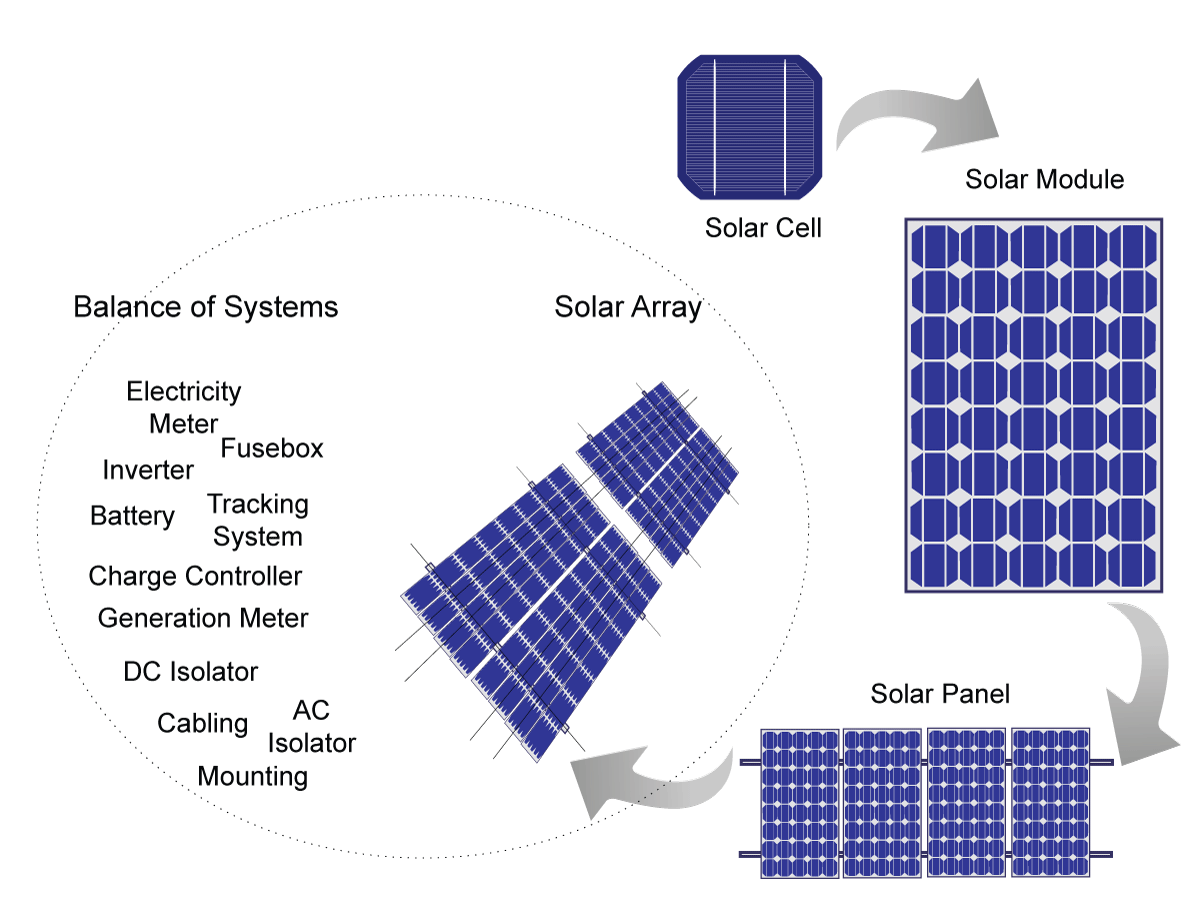
\includegraphics[width=350]{img/photovoltaic_system.png}
\caption{A Photovoltaic System}
\label{pv_system}
\end{figure}

A photovoltaic system is composed of two main elements, one is what is typically described as a solar array and the other are balance-of-system components. 

A solar array is usually composed of individual photovoltaic cells wired in series, called a string. This is done to increase the voltage produced by individual cells. The strings are then wired in parallel to increase the current. This collection of strings is then encapsulated in a weather-resistant housing and is what we typically refer to as a solar panel. These panels are then connected to one another to form a solar array. The connection can be done in either series or in parallel depending on the desired voltage or current of the system. 

Balance-of-system (BOS) components encompass everything that is not the solar panels or array. The BOS components include the array structure, solar tracker, connectors, AC and DC wiring, over-current protections, disconnects, interconnects, charge and system controllers, maximum power point trackers, batteries, inverters and any other accessories. The purpose of the BOS components is to integrate the solar system into the utility grid.

A photovoltaic inverter is an electrical device that converts the variable DC output of the solar panels to an AC frequency allowing it to be fed to the utility grid. Of all the BOS components, the inverter has historically had the most reliability problems. A international decade-long survey of photovoltaic systems indicated that a majority of failures, 65\%, were attributed to inverters\cite{Laukamp2002}. The same research also stated there appears to be ongoing reliability improvements, as the rate of failure declined over time. Even with these improvements, recent research confirmed that inverters continued to be the most likely causes of photovoltaic system failure\cite{Golnas2013}. 

Inverter reliability is essential for ensuring steady output of a solar system. When an inverter fails, it disables all photovoltaic cells upstream of it. This makes it the single largest potential source of productivity loss in a solar system. It is for this reason, a predictive maintenance process focused on the photovoltaic inverter can serve as a valuable mechanism for optimizing operational outputs. 

Yet, there are a number of difficulties in deploying such a process within this domain. Given its role as the device connecting the solar panels to the utility grid, the inverter contains most of the intelligence in a photovoltaic system\cite{Golnas2013}. However, this intelligence is minor and narrowly focused. At any given moment, an inverter records its electrical output in kilowatt hours (kWh) and possibly provides an error code if a malfunction has been detected\cite{SMA2012}. Unfortunately, these error codes are noisy and are not always present prior to an inverter failure. Even when an error code is present, it does not uniquely define a specific cause of failure. It, instead, expresses a symptom of failure, such as current leakage, over-voltage or software error, rather than the underlying cause. Furthermore, there is a tacit acknowledgment of the lack of causality between the presence of these error codes and inverter failure. This can be seen in most dashboards of solar systems which will report a count of the number of error codes that have occurred throughout the day. Thus, a single error is not seen as particularly severe and, as stated earlier, may not even occur prior to inverter failure. 

Additionally, communication errors are relatively common with system condition data, at a rate even higher than inverter failure\cite{Golnas2013}. This results in missing values being present in historical data. As these missing values are of electrical output and error logging, it results in confusion as to whether or not the system has experienced failure or not. It also makes it impractical to use interruptions in system conditioning data as a means of detecting failure. It is an obligation of system operators to provide logs for such downtime so that this distinction can be made. However, given their frequency, and their requirement for human intervention, this often does not occur. Yet, improvements of system network connectivity are likely to resolve this problem in the near future, both in terms of on-site data collection and continuous transmission.

The lack of robust system condition data poses a challenge in developing a predictive maintenance process. At its core, the lack of condition data stems from the modularity of design in photovoltaic systems. Every additional component not directly related to generating electrical output is viewed as an operational overhead, requiring cost-benefit justifications which often do not fit into profitability planning. As a result, the inclusion of accurate sensors which track reliability indicators like temperature and humidity at the inverter level are viewed as cost prohibitive additions and generally not included. This leads to informational sparsity in photovoltaic systems and especially in inverters. 

This can be contrasted with another alternative energy source, wind, which by design does not face such problems. A wind-turbine has roughly a hundred sensors that measure everything including ambient humidity, temperature, airflow and electrical current\cite{Ciang2008}. Of course, wind-turbines are self-contained and far less modular compared to a photovoltaic system. However, other industries, such as cloud computing, that have similar modular designs do not share the same sensor deficiencies. For example, the average cloud storage server rack contains more than a hundred temperature sensors, with each server averaging three\cite{Patel2003}. The key is that the monitoring requirement of a cloud computing server rack and a solar system are comparable. Yet, there is a substantial difference in the application of sensors to create a cohesive picture of health for each unit. The cloud storage industry clearly believing that system conditioning data is worth the overhead expense. 

As the industry matures and solar power becomes independently profitable, it is likely that it too will invest more heavily in condition-based monitoring of photovoltaic inverters\cite{Feldman2014}. However, this is not yet the case. Most sensors in a solar system are at the scale of solar park as a whole, not at the scale of an inverter. Thus, temperature, humidity and solar radiance data, assuming they are recorded at all, are provided by park level sensors. With large solar parks having multiple sensors installed. This is remarkably suboptimal, as solar parks at a utility-scale can encompass a large landmass, some exceeding a hundred square kilometers. A dozen sensors scattered among that landmass will undoubtedly produce a noisy signal regarding the health of any individual inverter. There are also attempts to reduce costs of sensors by employing satellite sensor data. However, this provides even worse resolution than park-level sensor data and thus even noisier signals regarding the health of an inverter.

While the system itself may not record a substantial amount of useful data, the humans working with the systems often do. This provides contextual information which can be used in the construction of a predictive maintenance process. 

System attributes are almost always kept complete and up to date. The make, model, installation date, location and other static data are recorded. Utility-scale solar companies often have warranty contracts with manufacturers which depends on the accuracy of this data\cite{Grigoryan2010}. This often includes offers to replace faulty elements within a specific time of purchase. 

Maintenance logs and failure history are usually kept but the level of detail depends on an organization's commitment and awareness of the utility of this data. Some companies chose not to employ maintenance logs at all, instead opting for run-to-failure operations. As the name suggests, components in the system are run until they fail and are then replaced. This is an suboptimal reactive approach, and also the most expensive form of maintenance. It leads to to increased downtime and higher costs of repair parts\cite{Mobley2002}. Companies that run-to-failure will usually still store accurate failure times for these components but not always. This can result in discrepancies between failure times and a lack of system electrical output leading to confusion about exact timing of any failure\cite{Laukamp2002}. Companies that invest in some level of preventative maintenance will keep logs which include what components were inspected and what, if any, corrective measures were taken. However, the level of detail of these logs varies highly. If kept, some degree of high-level root cause is almost always included. This may be at a level that is not sufficiently discriminating such as the use of "parts and material" or "external cause" as failure categories. Some companies, especially the large ones, do provide further context for these failures, but they are usually still fairly high level, such as "control software" and "AC contactor". However, limited willingness to engage in deep-failure analysis can dampen the value of collected information\cite{Golnas2013}.

As is clear, there are some significant hurdles to overcome in the development of a predictive maintenance process within the solar energy domain. However, as the industry matures and becomes increasingly self-sustainable it will undoubtedly correct many of these imperfections. 

\section*{Simulated Data and Model Justification}

The purpose of this section is to broadly lay out the simulated data set used throughout the remainder of the text and justify the use of a Bayesian time-to-event model. 

The simulated data uses the basic designs of a real-world photovoltaic system, but lacks the faults generated by poor data management, connectivity issues and other administrative errors. The data sources of several photovoltaic companies were used as the basis for the simulated data. For the sake of exposition, the data is a simplification of reality, in that it does not cover many of the possible externalities that arise in such a system. The purpose, after all, is to demonstrate how a predictive maintenance process can be developed rather than focusing on eliminating edge-cases. Furthermore, the use of simulated data provides the ability to iteratively construct a usable model and add complexity as required. 

It contains enough similar features to allow for it to be considered a reasonably representative data set. Five-hundred inverters unevenly clustered in five solar parks are generated. Each of the five-hundred inverters is provided with an ID, a model type, and a park. One generic failure mode is used. One which occurs within the first year of operation, representing sources of infant mortality commonly found in inverters\cite{Dhere2005}. The same type of process could just as easily applied to old age wear or any other failure mode. However, given that inverters expected lifetime is a decade, this would insert added complications related to technological innovation in that period which are beyond the scope of this text.


% <!-- The other failure mode is old age wear, which peaks within ten years of operation, on average. Admittedly, this is a pessimistic choice for a time frame given improvements in inverter reliability over the preceding decade. However, it is justified in that most current solar systems will still be making use of older components. -->

% <!-- The temporal granularity of the data is daily. A predictive maintenance process could be set up on an hourly, even second basis. However, the inability to act, not to mention the time required to refit the model, makes such such narrow intervals impractical. -->

Electrical output data is provided, with both trend and seasonality removed. Furthermore, error codes are provided. Two generic error codes are generated whose combinations are related to the aforementioned failure mode. Park level data is also provided. Temperature and humidity measurements are provided at the solar park level, which are combined into an extreme weather event count. 

%<!-- All of this data is then subject to feature engineering, to extract its relevant values for the modeling process. -->

%<!-- As time-dependent data requires a trajectory in time-to-event models, this data is heavily processed to extract  -->

Finally, maintenance logs are compressed into a single activity, related to component repair or replacement within a photovoltaic inverter. It should be stressed that replacement refers to subcomponents of the inverter, like capacitors, not the inverter itself. A count of the days since the last instance of such an activity is given.

From this description, it is clear that this simulated data could be infinitely more complex. In a real-world setting, there are a greater number of failure modes, error codes and maintenance activities. However, in order to derive the essence of predictive maintenance process, this level of simplification is justified. Additionally, a real-world context is unlikely to have a greater quantity of machine condition data, only further contextual information. Thus, this additional context simply increase the dimensions of the input but does not alter the heuristic required to produce a predictive maintenance process. 

There are numerous available techniques for generating predictions of remaining lifetime. However, most of these techniques require a greater volume of condition monitoring data than is available in an average photovoltaic system. The selection of Bayesian time-to-event analysis is based on a desire to optimally use the information that is available. 

The use of time-to-event models is an acknowledgment that any system's history informs the state of any other system at similar stages of deterioration. While other methods exist that could be used for the development of a predictive maintenance process, like multiclass classification models or multiclass logit models or regression trees, none of these methods operate well in a context with a limited amount of censored data. Yet, Bayesian methods make optimal use of this small amount of available data and can be adapted to deal with censoring. Furthermore, these methods provide valuable insight into the nature and composition of breakdowns. Thus, they provide valuable information that can be used for corrective and preventive purposes outside of the predictive process.


\section*{Extended Reading}

For an understanding of international energy policy and the role that solar power plays, the OECD's World Energy Outlook is a good place to start\cite{EIAOutlook2016}. For an in-depth, but dated, introduction to predictive maintenance, the reader is directed to Mobley\cite{Mobley2002}. For a general view of constructing predictive maintenance solutions in informationally rich domains, Microsoft has assembled an excellent step-by-step guide\cite{Uz2016}. For an overview of the reliability issues specifically related to photovoltaic systems, the reader is directed to Golnas\cite{Golnas2013} and Petrone\cite{Petrone2008}. 


% Maybe add alternative methods?
\chapter{Methodology}
\markboth{Methodology}{Methodology}

Time-to-event analysis/footnote{also known as survival analysis, reliability analysis and event history analysis} concerns itself with the modeling of the expected duration of time until an object experiences a well-defined event. This event is a transition between a finite number of possible states, such as from operational to non-operational or from alive to dead\cite{Andersen1992}. In this particular context, these states define the transition of a photovoltaic inverter from functional to failed.

To be able to model the time until these transitions, precision in describing phenomenon is needed, and for that, mathematics is required. The following chapter describes the mathematical narrative that underlies the construction, manipulation and estimation of Bayesian time-to-event models. It begins with the basic functions required to understand this class of models, their relationship, and role in defining time-to-event distributions. Then, censoring and truncation which are common characteristics of time-to-event data are examined. From these basics units, the Multiplicative Hazard Model for time-to-event analysis is formulated. Following this, a hierarchical model which describes shared risk, or Frailty is introduced. Finally, a description of the likelihood and model estimation with Hamiltonian Monte Carlo is given.



\section{Time-to-Event Functions}

The purpose of this section is to firmly root time-to-event analysis in the broader context of statistical modeling. It demonstrates the mathematical functions required to interact with this class of models, as well as providing their relationships. As this section is foundational, its content can be attributed to a diverse number of sources\cite{Aalen2008}\cite{Tableman2004}\cite{Klein2003}\cite{Kleinbaum2005}\cite{Cleves2008}\cite{Rodriguez2007}.

Begin, by defining $T$, a continuous non-negative random variable with an unknown distribution representing the time until a well-defined event. As it is a time, its support is constrained to all positive real numbers, ($T \ge 0, T \in \mathbb{R}$). Further, define $t$, to be the realization of this random variable at a specific point in time.

A familiar way of describing a probability distribution is to use probability density function (pdf) and cumulative distribution function (cdf). The pdf is the relative likelihood of a random variable taking a particular realization.

$$f(t) = \Pr(T = t)$$

The cdf defines the probability that a random variable will take on a value less than or equal to some realization. Thus, it defines a range of outcomes across the random variable.  

$$F(t) = \Pr(T \le t) = \int^t_0 f(x) dx $$

In the time-to-event context, the cdf of $T$ may not be particularly useful as the variables of interest usually take on values greater than some realization. This is because in most cases, $T$ will be greater than the value observed, $t$. Fortunately, by definition, a random variable must sum to one and the complement of the cdf can be established through subtraction.

$$S(t) = P(T \ge t) = 1 - F(t) = \int^{\infty}_t f(x) dx$$

This returns the survival function\footnote{also denoted as the reliability function $R(t)$} which is the probability
that the well-defined event occurs after a specific point in time. It is considered the survival function because it provides the probability of surviving beyond an observed time, $t$. Clearly, if the event occurs after a specific time, then the event has not yet occurred. As the event is death or failure, it is implied that the object of interest has survived up to that point.

As the survival function is the complement of the cdf, it inherits its properties. It is monotonically decreasing, with $S(0) = 1$ and $S(\infty) = \lim_{t\rightarrow \infty}S(t) = 0$. This formalizes the notion that when the event in question is failure, in the beginning all systems are operational, but given a long enough time frame all systems will eventually fail.

While the survival function focuses on the event not occurring, the hazard function focuses on the event occurring. The hazard function\footnote{also known as the conditional failure rate, intensity and force of mortality} is the instantaneous rate of failure given that failure has not yet occurred.

$$ h(t) = \lim_{\Delta t \rightarrow 0^+} \frac{P(t \le T < t + \Delta t | T \ge t)}{\Delta t} = \frac{f(t)}{S(t)} $$

It provides the potential of the event occurring within the next limiting time interval, assuming it has not taken place until now. It should be stressed, that this function does not return a probability, rather a rate ( $\frac{P}{\Delta t}$ ). It must be non-negative, such that $h(t) \ge 0$, and can take on values greater than one $[0, \infty)$.

The hazard is far more useful from a practical perspective than the other constructions. The conditional formulation is especially important, as the hazard defines the risk only after excluding the prior occurrence of the event. This makes it a more natural expression of what is generally asserted as the risk of an event in time, which implicitly presupposes that the event has not yet occurred.

Numerically, the hazard is clearly linked to the future occurrence of the event. When the hazard is zero, the risk of the event occurring in the next moment is also zero. Conversely, when the hazard is infinite, the risk of the event occurring the next instance is near certain.

The hazard is a limiting rate, and is concerned with the event within an instantaneous interval. At times, it is beneficial to understand that potential across an interval of time.

$$ H(t) = \int^t_0 h(u) du $$

This is the cumulative hazard function. It measures the total amount of risk that has been accumulated up to time $t$. The cumulative hazard can be understood as the number of times we would expect to observe the event in a given period of time, assuming the event were repeatable.

The relationship between the hazard and cumulative hazard is especially important in providing intuition. The hazard is a rate is defined in $\frac{1}{t}$ units. Whereas the cumulative hazard sums across those $\frac{1}{t}$ units. For example, if a rate of a particular event was ten, and five units of time passed, then fifty events would be expected within those five units. It is important to note, that this logic is one-directional and is based on an assumption of a constant hazard rate over the five units of time. There is nothing that makes this generally true. Thus, when starting with a cumulative hazard of fifty, it is possible that the hazard rate is fifteen, five, ten, five, and fifteen, respectively, for each of the five units of time. 

The pdf, cdf, survival, hazard and cumulative hazard functions all uniquely define the process generating time-to-event data. As a result, it is possible to transform any of these functions into any other. This is useful because it provides insight into the relationships among the functions but also because it allows for the use of the easiest constructions in modeling.

It is generally true that any pdf can be expressed as a derivative of its cdf. As a result, the survival function also provides a route back to the pdf. The negative derivative of the survival function returns the pdf. Such that the pdf can be redefined as follows:

$$ f(t) = \lim_{\Delta t \rightarrow 0^+} \frac{\Pr(t \le T < t + \Delta t) }{\Delta t} = \frac{d F(t)}{dt} = - \frac{d S(t)}{dt}$$

The hazard function and survival function are also intimately related to one another. From the above identity, it can be seen that the pdf in the definition of the hazard can be replaced with the negative derivative of the survival function. The same can be done in the definition of the hazard. It is then clear that the hazard can be expressed as the negative derivative of the logarithm of the survival function.

$$ h(t) = \frac{f(t)}{S(t)} = - \frac{d S(t) / dt }{S(t)} = - \frac{d \ln \left( S(t) \right) }{dt} = - \frac{d}{dt} \ln S(t)$$

The above identity can also be used to express the cumulative hazard. Integrating from a starting time until a specific time, demonstrates that the cumulative hazard can be defined as the negative logarithm of the survival function.

$$ H(t) = \int^t_0 \frac{f(u)}{S(u)}du = - \int^t_0 \frac{1}{S(u)} \left( \frac{d}{du} S(u)\right) du = -\ln S(t) $$

Whatever transformation is expressed in terms of logarithms, can be reversed through exponents. Thus, the survival function can be defined as the exponent of the negative integral of the hazard function, or the negative cumulative hazard.

$$ S(t) = \exp \left (- \int_0^t h(u) du  \right ) = \exp(-H(t)) $$

This allows for the conversion of a cumulative hazard back into a probability. Given the earlier example of a cumulative hazard of fifty the survival probability can be determined: $S(t) = \exp(-50) = 0.19 \cdot 10^{-22}$ which is a near zero probability of survival.

The pdf can also be expressed in terms of the exponent of the negative integral of the hazard function, or the cumulative hazard.

$$ f(t) = h(t) \exp \left (- \int_0^t h(u) du  \right ) = h(t) \exp(-H(t)) $$

As can be seen, regardless which of the functions are available, it is possible to produce a transformation which will return all the others. This is useful because generally, the hazard or survival time rather than the density are the objects of interest.

All of these functions can be conditioned to only extend to events that occur after a particular point in time. This is useful when dealing with lifetimes where the system has not been observed from the time it became operational. It is also useful when constructing expressions about particular intervals of time\cite{Cleves2008}.

$$ h(t|T > t_0) = h(t) $$

$$ H(t|T > t_0) = H(t) - H(t_0) $$

$$ F(t|T > t_0) = \frac{F(t) - F(t_0)}{S(t_0)} $$

$$ f(t|T > t_0) = \frac{f(t)}{S(t_0)} $$

$$ S(t|T > t_0) = \frac{S(t)}{S(t_0)} $$

One final construction of interest is the expected residual lifetime. This is the amount of life a particular system is expected to have given it has survived up to a specific time ($t_0$).

$$ E(t|T > t_0) = \int^\infty_{t_0} S(t) dt \cdot \frac{1}{S(t_0)} $$


\section{Common Lifetime Distributions}

Any continuous distribution defined over the positive numbers can be used as a lifetime distribution. This section briefly covers several commonly used distributions for modeling lifetimes and provides justifications for their use. The exponential, Weibull, Gompertz and Gamma are described.

The simplest lifetime distribution can be defined by assuming a constant hazard rate ($\lambda$) over time.

\begin{align*}
h(t) = \lambda \tag{ $\lambda > 0$}
\end{align*}

As was demonstrated earlier, this can be transformed into a survival function by exponentiating the integral of all values from start until $t$. As the hazard is constant, this will simply be the exponent of the constant multiplied by the number of intervals present.

$$ S(t) = \exp \left (- \int_0^t \lambda\; du  \right ) = \exp (- \lambda\; t )$$

If transformed into a density, its characterization becomes immediately apparent.

$$ f(t) = - \frac{d S(t)}{dt} = \lambda\; \exp(- \lambda\; t) $$

This is the functional form of exponential distribution. It is useful in two areas in time-to-event analysis. First, it can be used to model events whose likelihood of occurrence does not vary with time. It can model systems that are not affected by wear or aging. For example, the exponential distribution is a suitable model for the release of particles from radioactive material\cite{Jowett1958}. However, these types of events are relatively rare in industrial settings. There are very few systems that do not experience some changes as a result of their length of operation. The second area of use for the exponential distribution is the discretizing of time. Time is continuous but data is not. Thus, there is a need to define how continuous time behaves across recorded intervals. The most consistently used assumption is that the hazard does not change within any given interval. If these intervals are sufficiently small such an assumption is perfectly valid.

Most lifetime distributions arise as generalizations of the exponential. They provide a more elaborate construction for the hazard over time based on some underlying logic.

The Gompertz distribution is a generalization of the exponential that introduces an exponential effect in the hazard over time.

\begin{align*}
h(t) = \lambda \exp(\varphi t) \tag{ $\lambda > 0, \varphi \in (-\infty, \infty) $}
\end{align*}

The formula was originally derived to characterize the exponential rise in death rates in humans between sexual maturity and old age\cite{Wienke2010}. It introduces a shape parameter $\varphi$ which controls the rate of change of the hazard over time. When $\varphi < 0$ the hazard declines over time. This can be used to model component "burn-in", which is the time shortly after beginning operations where mechanical parts often experience early failures. Conversely, when $\varphi > 0$ the hazard increases over time. This can be used to model end of life failure. If $\varphi = 0$, the Gompertz reduces to an exponential distribution. When the Gompertz hazard is not constant, it is always increasing or decreasing over time. This makes it particularly attractive when it is clear that operational time is the greatest force of mortality.

The Weibull distribution also introduces an exponential effect in the hazard function over time. Yet, it does so in a more flexible manner.

\begin{align*}
 h(t) = \lambda \nu t^{\nu - 1} \tag{ $\lambda >0, \nu > 0$ }
\end{align*}

It introduces a shape parameter $\nu$ that also controls the increase or decrease of the hazard over time. It is more flexible than the Gompertz in that it is capable of modeling hazards that increase initially, but whose rate of increase declines over time when $(0 < \nu < 1)$. The Weibull also has a common alternative parameterization, which is common in many software packages.

\begin{align*}
h(t) = \frac{\alpha}{\sigma} \left (\frac{t}{\sigma}  \right )^{\alpha - 1} \tag{$\alpha > 0, \sigma > 0$}
\end{align*}

This parameterization defines a shape, $\alpha$, and a scale, $\sigma$, parameter. These parameters are equivalent to the rate, $\lambda$ and shape, $\nu$, in the earlier form such that, $\lambda = \sigma^{-\alpha}$ and $\nu = \alpha$.


The Weibull distribution was originally developed to assess the catastrophic failure of materials. No material is perfectly uniform and all contain irregularities at some scale. These irregularities such things as pores, mineral inclusions or micro-cracks are distributed throughout the material. While under pressure any one of these irregularities can induce failure. As a result, the Weibull formalizes the notion of the "weakest link"\cite{Rinne2008}. It is the minimum of any collection of independent identically distributed random variables. This is important in the reliability of complex systems as different causes of system failure compete with one another and the first cause will result in the failure of the entire system\cite{Quinn2010}.

Gamma distribution, like those before it, is also a generalization of the exponential. However, its justification for use as a lifetime distribution is a bit more involved. A system may be exposed to a number of shocks, each of which are exponentially distributed. The system may be resilient to each shock up to a threshold, upon which it fails. The sum of each of those exponentially distributed shocks is gamma distributed\cite{Tso2010}. The hazard function is as follows:

\begin{align*}
h(t) = \frac{\lambda^k t^{k-1} \exp(-\lambda t)}{(1 - I_k(\lambda t)) \Gamma(k)} \tag{$ k>0, \lambda > 0 $}
\end{align*}

With $k$ being the number of exponentially distributed shocks that occur prior to system failure. As can be seen the hazard is quite complex, making use of both the gamma function $\Gamma(k)$ and the incomplete gamma integral $I_k(\lambda t)$.

$$ \Gamma(k) = \int_0^\infty x^{k-1} \exp(-x) dx \qquad I_k(x) = \frac{\int_0^x s^{k-1} \exp(-s) ds}{\Gamma(k)} $$

In traditional model fitting techniques, the incomplete gamma function imposes numerical problems for parameter estimation\cite{Wienke2010}. This has resulted in the gamma function not finding widespread application in the modeling of lifetimes. Recently there has been a resurgence in the use of the Gamma distribution, especially in the Bayesian context where optimization problems are less of a hurdle to application. Additionally, hierarchical modeling makes use of the Gamma distribution as method of modeling unobserved heterogeneity among groups of lifetimes, a subject discussed further in a later section.


Other lifetime distributions exist. However, the preceding cover the overwhelming majority of common parametric distributions used to model lifetimes. Further, while all the distributions described have mathematical and contextual justifications for their use in specific contexts, these are not always of utmost importance. Historically, the fact that a distribution provides an accurate fit for the data has been an overriding justification in many applications\cite{Marshall2007}. Furthermore, it should be stressed, regardless of which distribution is selected to model lifetimes, its adequacy should be checked. A topic which will be returned to in the following chapter.


\section{Truncation and Censoring}

Truncation and censoring are defining elements of time-to-event models. The functions that have been described so far have assumed an environment where the waiting time until an event is fully observed. In most real-world applications, however, it is impractical to wait until all systems in the population fail. Therefore, time-to-event models usually exist in incomplete information. Truncation and censoring provide mechanisms to formalize how that state of limited information affects the model. The following section describes how truncation and censorship affect data, provide several standardized schemes for censorship and how the phenomena can be expressed mathematically.

Truncation refers to when values outside a particular bounds are entirely omitted. Simply put, in a truncated data set, systems are only observed if they have survived up to a particular point in time. Truncation is less common in reliability contexts but does still occur. For example, if systems' lifetimes were recorded only if they had failed after a particular date. Then those systems that had failed prior to that particular date would not be recorded and thus truncated\cite{Hong2009}.

Censoring refers to when values are only known to occur within a particular range. In time-to-event analysis it is common to examine events that occur in the future. As a result, the exact timing of an event may not be known. Yet, its the direction from the observed value, is known. This observation still provides partial information about the timing of an event but not as much as a fully observed event. 

The difference between censorship and truncation can be viewed as the difference between known-unknowns and unknown-unknowns. If truncation exists in a data set, observations are omitted from that data set and it is impossible to determine if those observations included events or not. With censoring, the source of the observations is retained, but there is uncertainty as to the exact timing of the observation. Both have detrimental effects on model fit, but the effect of truncation results in substantially greater bias.

There are different types of censoring depending on which segment of the data is missing. If the event in question is missing because it is in the future, right-censoring is said to present. If an event has already occurred but the object was not observed at the time, left-censoring is said to present. Interval censoring occurs when an event is known to have occurred within a specific range of times, but its exact timing is not known. 

Censoring is also categorized depending on the mechanism leading to observations being censored. Different schemes exist, mainly from the literature on clinical trials, which define mechanisms where censorship occurs. This includes, if the event occurs after a particular end date (Type I) or if it occurs after a specific number of events have been observed (Type II). However, more common, is random or non-informative, censoring. As the name suggests, this is when censoring occurs randomly and is independent of failure times.

Censoring can be operationalized by augmenting the underlying distribution of the time until our well-defined event, $T$. First, a binary random variable $d$ is defined. This variable takes on a value depending on what is observed at time $t$. If at time $t$ the event has occurred, then $d$ takes on the value of one. If at time $t$ the event has not yet occurred and is therefore censored, $d$ takes on the value of zero. With the introduction of $d$ it is clear that $T$ is not being directly observed. Rather, another distribution which contains censoring times $C$ is interfering. What is being observed is instead the minimum of both the failure times and the censoring times, which we denote as $Y$.

$$  Y_i = \min(T_i,C_i) \qquad \text{ and } \qquad d_i = \left\{\begin{matrix} 1 \text{ if } T_i \le C_i\\ 0 \text{ if } C_i < T_i \end{matrix}\right. $$

This provides a route to expressing what is actually being observed within a time-to-event data set, which is a combination of two distributions, one of real lifetimes, the other of censoring. 



\section{Hazard Modeling with Covariates}

Hazards provide the means by which to assess the risk status of any particular system in the population over any given interval. This makes it an ideal metric through which to model the probability of failure. The constructions discussed so far have had an implicit assumption. Namely, that the lifetime distribution $T$ arises from systems under identical conditions. Effectively, this implies that the population from which these lifetimes are derived is homogeneous. In practice, it is obvious that not all systems will be subject to the identical risks and conditions. Systems will have distinct manufacturers and locations, not to mention being exposed to an assortment of risks due to different operating conditions. However, to enable this diversification of lifetimes, a method to integrate covariates that formalizes this diversity is needed. The following section describes the Multiplicative Hazard Model which provides a means to express this diversity, and demonstrates several extensions to the model to allow for more complex covariates.

To incorporate covariates into the model of lifetimes, a function, $g(\cdot)$, that permits offsets for each individual system, $i$, is required\cite{Cleves2008}\cite{Tableman2004}.

$$ h_i(t|\textbf{x}_i) = g(t, \beta_1 x_1 + \dots + \beta_m x_m)  $$


This function should alter the hazard by a given vector of covariates, $\textbf{x}_i = (x_1, \dots, x_n)$, for each individual system, and a shared vector of coefficients $\boldsymbol\beta = (\beta_1, \dots, \beta_m)$. Together, this is a linear model, $\boldsymbol\beta^T \textbf{x}_i = \beta_1 x_1 + \dots + \beta_m x_n$.

There are numerous routes to finding the function $g(\cdot)$. Yet, it is important to keep in mind the constraint on the original hazard. Any hazard must be positive, this means that the output of $g(\cdot)$ must also be positive. There is nothing to prevent the linear model from producing a negative output. However, a simple logarithmic transformation can prevent this outcome.

\begin{align*}
\ln(Y) = \boldsymbol\beta^T \textbf{x}_i \\
Y = \exp(\boldsymbol\beta^T \textbf{x}_i)
\end{align*}

Once the positive output hazard is ensured, there remains the question of the functional form of $g(\cdot)$. The most common solution is to treat the linear model as acting multiplicatively on a shared baseline hazard, $h_0(t)$.

$$ h_i(t|\textbf{x}_i) = h_0(t) \exp(\boldsymbol\beta^T \textbf{x}_i) $$

The baseline hazard, $h_0(t)$ is the common hazard when all covariates are zero, as $\exp(0) = 1$. In this way, it is the considered the baseline as it occurs prior to considering any additional variables\cite{Kleinbaum2005}. Note, the linear predictors do not contain an intercept term and rather begin with $beta_1 x_1$. This is because the baseline hazard already acts as an intercept for the model. The absence of the effect of the covariates would simply be the baseline hazard at that time.

This is the simplest form of the Multiplicative Hazard Model\footnote{Also known as the Cox Regression Model}. Whereas in a standard linear model, the estimated parameter value implies a linear change in every individual's fitted value, in this Multiplicative Hazard Model, a change in an estimated parameter implies a proportional shift in each individuals hazard at all time points\cite{Mason2015}.

There is nothing deterministic about the use of multiplication as the form of $g(\cdot)$. The linear model could have just as easily been added rather than multiplied. There exists an entire class of additive hazard models\cite{Lin1997}. However, they are far less common in practice, mainly due to difficulties fitting these models\cite{Boshuizen2010}. This lack of application has led to a smaller quantity of available literature.

This multiplicative construction separates the baseline hazard, $h_0(t)$ from the linear model, $\boldsymbol\beta^T \textbf{x}_i$. This allows for the baseline hazard and linear model to be estimated separately of each other. This greatly simplifies the fitting process. Furthermore, it allows for the comparison of the effect of any set of covariates through a proportion, known as a hazard ratio.

$$ \frac{h(t|x_1)}{h(t|x_2)} = \frac{h_0(t) \exp(\boldsymbol\beta^T x_1)}{h_0(t) \exp(\boldsymbol\beta^T x_2)}  = \exp( \boldsymbol\beta^T(x_1 - x_2) )$$

In the above ratio, it is clear that time, $t$, along with the baseline hazard, $h_0(t)$, are factored out of the final construction. In this form, the hazard is not dependent on time, just on the effect of the covariates. This specific form of the Multiplicative Hazard Model is known as the Proportional Hazards Model.

The feature that allows for time to be factored out of the model is also a limitation. In separating the baseline hazard from the linear model, a hard assumption is made about the nature of the covariates. Specifically, that they must be time-invariant, or remain static through time. This does apply to many types of covariates that can specify the level of risk to which a system is exposed, like its location, manufacturer or whether it is part of a control group. 

Fortunately, feature engineering methods can be used to construct variables that are time-invariant from ones that are time-dependent in raw data. This allows for any variables to be used within these models. Furthermore, it is possible to extend the Multiplicative Hazard model to explicitly include both time-dependent effects and time-varying covariate\cite{Dekker2008}. However, due to the complexity of the model fitting mechanisms of these constructions, especially with Frailties, these are beyond the scope of this text. 


\section{Frailty}

So far, all the models described have implicitly assumed that given a set of covariates, the resulting lifetimes are independent and drawn from the same underlying distribution with the same parameters. In practice, such an assumption, while useful, is rarely realistic. Thus, there is a need to extend the model further to allow for correlation between observations. This is done through the introduction of a Frailty into the model.

A Frailty\footnote{Also known as a mixed/random effect, longevity factor, susceptibility or liability. When introduced into the model, it makes a mixed hazard model, or a hierarchical hazard model} is an unmeasured random effect that is incorporated into a hazard function to account for heterogeneity in the population\cite{Hosmer2008}. This unobserved random quantity impacts the hazard function multiplicatively.

$$ Z\cdot h(t) $$

At its core, the Frailty provides a means by which to account for the fact that data often contains groupings or clusters of similar observations even if not explicitly modeled, leading to dependence among observations. This dependence implies some unknown correlation structure within and between these groups. The inclusion of a Frailty provides a method to model this dependence. It assumes conditional independence among lifetimes given the Frailty. This shared Frailty is the source of dependence within a group\cite{Wienke2010}. For example, inverters clustered within solar parks will exhibit similar lifetimes as a result of being exposed to similar conditions. Furthermore, inverters of a similar type or manufacturer are also likely to share attributes that lead to correlations in their lifetimes. This provides valuable information about the health of units within these groupings allowing for more accurate prediction of their lifetimes.

Yet, much of these similar conditions are unlikely to be fully captured by the covariates in the model. This omission occurs when relevant covariates cannot be observed or are too costly to observe. It is impossible to collect all the risk factors that contribute to failure. There is rarely awareness of all contributing factors, either because their relevance is not known or because there is a lack of means to measure them. This is especially the case for complex electronic systems whose components interact with one another as well as the environment. The cost of observation is of particular relevance to the photovoltaic domain, as the inclusion of relevant data is limited by financial constraints.

The form of the frailty determines how correlation structure is modeled. A Frailty is introduced into the Multiplicative Hazard Model as follows:

$$ h_i(t|\textbf{x}_i, Z_i) = Z_i \cdot h_0(t) \exp(\boldsymbol\beta^T \textbf{x}_i)  $$

Here, $Z$, is defined as a non-negative random variable, with some distribution, $\mathfrak{g}(\cdot)$, varying across the population\cite{Wienke2010} with $Z_i$ being the realization of the Frailty for each individual system. Generally, the Frailty distribution is standardized, resulting in an average value equal to one, $\mathrm{E}[Z] = 1$, and a variance parameter that is estimated from the data, $\text{Var}(Z) = \theta$.

It is important to distinguish between the frailty itself and the random effect, $b_i^t$:  

\begin{align*}
h_i(t|\textbf{x}_i, Z_{i}) = h_0(t) \exp(\boldsymbol\beta^T \textbf{x}_i + b_i^t z_i)
\end{align*}

Where $Z_{i} = \exp(b_i^t z_{i})$ and clearly when $b_i = 0$ then $Z_i = 1$. This illustrates that the multiplicative effect the Frailty intends to model can alternatively be viewed as an additional covariate in the linear model. 


As the average value of the Frailty is set to one, divergences from the average characterize the effect on the hazard. Individual systems with Frailties greater than one will have a higher than average hazard, implying they are more frail. Meanwhile, individual systems with Frailties less than one will have lower than average hazard implying they are less frail. Those that are more frail will die earlier than those that are less frail.

Estimating a regression model without the introduction of random effects can bias the resulting predictions if individual observations are not truly independent. In time-to-event data, this issue is compounded by temporal effects. Individual systems that are more robust will almost certainly live longer and produce more data. The population hazard declines as a result of high-risk individuals failing, but the individual hazard may continue to increase. This systematic observation of the most robust individuals will skew the computation of the average hazard. Thus, an estimate of the individual hazard rate without taking into account unobserved Frailty will underestimate the hazard function to an increasingly greater extent as time goes by\cite{Aalen2008}.

The estimation of the variance parameter, $\theta$, describes the degree of diversity in baseline hazard of a population. A large $\theta$ implies a high degree of heterogeneity as lifetimes deviate heavily from the average value of one. Conversely, a small $\theta$ implies the homogeneity of lifetimes as each one will be heavily concentrated near the average value.


In the above construction, the Frailty is introduced in such a way that the entire population of systems is covered by a single distribution. In practice, it is more useful to estimate a Frailty for each distinct group within the population, as follows:

$$ h_{ij}(t|\textbf{x}_i, Z_j) = Z_j \cdot h_0(t) \exp(\boldsymbol\beta^T \textbf{x}_{ij})  $$

Here, a Frailty of a collection is introduced and each distinct group $j$ is composed of a total of $k$ distinct groups. A random variable, represents the collection, $Z_j = (z_1, \dots, z_k)$. A collection is defined as a set of groups that all share a common characteristics. To be properly defined, a collection should be mutually exclusive and exhaustive given the data. For example, there can only be a finite number of parks within which inverters reside. Each park makes up a distinct group, and all of the parks make up the collection. With this structure, it is possible to estimate the Frailty, and thus the level of heterogeneity for each group. The interpretation of the Frailty and its variance are identical to what has been described previously, except localized to each distinct group. This can be extended further to allow for as many different collections as is required, simply by introducing additional Frailties into the model multiplicatively. It should be noted, the multiplicative introduction of further Frailties implies independence between lifetimes of different collections. In fact, the lifetimes of individual systems are conditionally independent given the vector of Frailties. 


Any distribution which is positive and possesses a mean can be set to one, can be used as the Frailty distribution, $\mathfrak{g}(\cdot)$. The most commonly used distribution is the Gamma. It is utilized due to its flexibility in modeling positive outcomes as well as the ease with which it allows for the expression of all required formulas\cite{Wienke2010}. The density of the Gamma is given as follows:

\begin{align*}
f(t) = \frac{\lambda^k t^{k-1} \exp(-\lambda t)}{\Gamma(k)} \tag{$ k>0, \lambda > 0 $}
\end{align*}


As stated earlier, the goal here is to fix the average Frailty to one and estimate the variance. This can be done the following way:

\begin{align*}
\mathrm{E}[Z] = \frac{k}{\lambda} = 1 \tag{$ k = \lambda $}
\end{align*}


\begin{align*}
\mathrm{V}[Z] = \frac{k}{\lambda^2} = \frac{1}{\sigma^2} \tag{$ k = \lambda $}
\end{align*}


The restriction of $k = \lambda$ is made to ensure that the average Frailty is equal to one. Through this restriction we note that the variance is now, by definition, $\sigma^2 = \frac{1}{\lambda}$. This leads to the conditional density of the Gamma distributed Frailty:

$$ f(z) = \frac{1}{\Gamma(\frac{1}{\sigma^2})} \left (\frac{1}{\sigma^2}  \right )^{\frac{1}{\sigma^2}} t^{\frac{1}{\sigma^2} - 1} \exp(-\frac{t}{\sigma^2}) $$

This density can be transformed into a unconditional survival function and consequently the into the unconditional density and hazard using the following formulas:

$$ f(t) = \frac{h_0(t)}{(1+ \sigma^2 H_0(t))^{\frac{1}{\sigma^2}+ 1 } }$$

$$ S(t) = (1 + \sigma^2 H_0(t))^{- \frac{1}{\sigma^2}}$$

$$ h(t) = \frac{h_0(t)}{1 + \sigma^2 H_0(t)} $$


The corresponding hazard and cumulative hazard can be replaced with the appropriate lifetime distribution. For example, let $h(t) =  \frac{\alpha}{\gamma} \left (\frac{t}{\gamma}  \right )^{\alpha - 1}$ be Weibull distributed baseline hazard with a Frailty following a Gamma distribution $Z \sim \text{Gamma}(\frac{1}{\sigma^2}, \frac{1}{\sigma^2} )$. Thus, the unconditional survival and hazard functions are given by the following expressions:

$$ S(t) = \left (1 + \sigma^2 \left (\frac{t}{\gamma}  \right )^{\alpha}  \right )^{-\frac{1}{\sigma^2}} $$

$$ h(t) = \frac{\frac{\alpha}{\gamma}\left (\frac{t}{\gamma}  \right )^{\alpha - 1}}{1 + \sigma^2 \left (\frac{t}{\gamma}  \right )^{\alpha} } $$

Where $\sigma^2$ represents the variance of the Gamma distributed Frailty.

There are several important issues that should be kept in mind when introducing Frailties to time-to-event models. A Frailty is assumed to be constant over time. If the random variable $Z$ is introduced as a Frailty into the Multiplicative Hazard Model, then the estimation of $Z$ is fixed for all time points. However, this does not mean that Frailties experience no temporal effects. This can be seen when the conditional expectation and variance of the Frailty $Z$ are derived:

$$\mathrm{E}[Z|\textbf{x},  T > t ] = \frac{1}{1 + \sigma^2 H_0(t) \exp(\boldsymbol\beta^T \textbf{x})} $$

$$ \mathrm{V}[Z|\textbf{x},  T > t ] = \frac{\sigma^2}{(1 + \sigma^2 H_0(t) \exp(\boldsymbol\beta^T \textbf{x}))^2} $$

Two things of note can be understood from the above. First, individuals dying at time $t$ will have a higher mean Frailty compared to survivors. This is because the cumulative hazard in the denominator increases as time goes on. Second, the variance of Frailty declines over time. This implies that early failures reduce the heterogeneity of of the population over time. However, the ratio between the average Frailty and its variance remain constant over time implying that the population does not become more homogeneous relative to the average in time\cite{Wienke2010}.

The introduction of a Frailty, at any level, will invalidate the Proportional Hazards property\cite{Kleinbaum2005}. The property, explained in the previous section, allows for the a comparison between any set of covariates through a simple proportion. However, with the introduction of the Frailty, any sets of covariates now require the computation of a temporal effect, such that:

$$ \frac{h_1(t)}{h_2(t)} = \frac{1 - \sigma^2 H_0(t)}{1 - \sigma^2 H_0(t) \exp(\boldsymbol\beta)} \exp(\boldsymbol\beta) $$

The ratio of specific population hazards is generally not time-invariant. This can be seen from the above equation, the hazard ratio is a decreasing function, unless there is no difference between groups or the Frailty is not relevant. The reason for this are, again, the alteration of the hazard rate in the population as high-risk individuals fail earlier leading to a lower average hazard rate over time.

There are significant advantages to using a parametric baseline hazard when introducing Frailties into a Multiplicative Hazards Model. The most important consequence of such a combination is that it enables the explicit description of the evolution of a Frailty over time. Without a parametric form it is difficult to describe how 

In a traditional context, the values of $Z_i$ are not estimated for each individual system within the population. The reasoning for this is relatively simple. An estimate of a $Z_i$ for each individual system, $i$, would require $N$ parameters. This would result in more parameters in the model than there are observations, leading to an over-saturated model. Furthermore, the estimation of individual Frailties are usually less important than group Frailties and variances. These provide useful estimates of the degree to which these groupings affect survival times, as well as identify patterns among those groups. That said, this traditional restriction is loosened in the context of Bayesian estimation where an estimation for $Z_i$ can be sampled.




\section{Model Likelihoods}

The likelihood is a function of the parameters of a statistical model given data. Its formulation is the means by which the appropriate mathematical abstraction is selected after data has been observed. In this section, likelihoods for the models developed so far are formulated. First in the simplest cases, then with the model additions.

Generally, a parametric model is fit by finding the maximum values for a set of parameters, $\theta$, of its probability density function, $f(\cdot)$, given a vector of data, $T = (t_1, \dots, t_n)$. This process is encapsulated in Maximum Likelihood Estimation (MLE):

\begin{align*}
\displaystyle \arg \max _{\theta }{\mathcal {L}}(\theta | T) &= \arg \max _{\theta }f(T|\theta ) \\
{\mathcal {L}}(\theta | T) = \Pr(T | \theta) &= \prod_i f_{\theta}(t_i)
\end{align*}

In the time-to-event context, there is an added complication. As noted earlier, this type of data often features censoring and truncation. When non-informative right-censoring is present, it is required to extend the likelihood. The data, $T$, is now input as a pair, $(y_i, d_i)$. The $Y$ random variable is defined as the minimum of the actual and censored lifetime. It represents the observed lifetimes found in the data. A binary random variable, $d$, is introduced to make explicit when censoring occurs. The likelihood is altered as follows:

$$ \mathcal {L}(\theta) = \prod^n_i f(y_i)^{(d_i)} S(y_i)^{1 - d_i} $$

The probability density function, $f(y_i)$, of the parametric distribution is still present in the above equation, much like in the standard likelihood. However, its contribution is now controlled by the $d$ random variable. When the variable $d$ equals one, it implies a failure event and the likelihood is evaluated in the general way. However, when $d$ is zero,  censoring occurs and the likelihood evaluates instead the survival function, $S(y_i)$, which implies the object has survived up to that particular point in time. The combination provides information about both observed events and about yet to be observed events. 

Given the identities found at the beginning of this chapter, it is possible to transform the joint likelihood to make use of hazards.  Such that the likelihood becomes:

$$ \mathcal {L}(\theta) = \prod^n_i h(y_i)^{d_i} \exp(-H(y_i)) $$

This generally provides easier functions to work with when constructing the likelihood. It should be noted that hazard estimation is restricted here to only include parametric forms. It is incredibly common to not make parametric assumptions about the baseline hazard. There is a large body of research into non-parametric baseline hazard estimation, including the Kaplan-Meier and Nelson-Aalen estimators. If contrasting the effect of covariates is the predominant purpose of the model, semi-parametric or non-parametric methods are often preferred. However, the structure of the baseline hazard has substantive implications for the ability to understand the model and predict. This is especially the case when Frailties are involved as parametric hazards aide in understanding the evolution of group hazards over time. Furthermore, non-parametric methods lack the ability to forecast future hazard rates beyond the last failure time, as any value beyond the last time is simply undefined. That said, the parametric form is not without its price, namely it is an assumption about the evolution of lifetimes which must be verified to be used.

The likelihood for the censored model can be extended to include covariates. First, recall the Multiplicative Hazards Model:

$$ h_i(y|\textbf{x}_i) = h_0(y) \exp(\boldsymbol\beta^T \textbf{x}_i) $$

In this case the data is input as a triple, $(y_i, d_i, \textbf{x}_i)$ as the covariates are also introduced. The likelihood for this function is as follows:

$$ \mathcal {L}(\theta) = \prod^n_i \left (h_0(y_i) \exp(\boldsymbol\beta^T \textbf{x}_i)  \right )^{d_i} \exp(-H_0(y_i) \exp(\boldsymbol\beta^T \textbf{x}_i)) $$

The introduction of a univariate Frailty into the Multiplicative Hazard Model is straight-forward. As stated earlier, the Frailty model can be generally stated as:

$$ h_{i}(y|\textbf{x}_i, Z) = Z_i \cdot h_0(y) \exp(\boldsymbol\beta^T \textbf{x}_{i})  $$

Thus, the likelihood with univariate Frailty and non-informative right censoring simply expands to:

$$ \mathcal {L}(\theta) = \prod^n_i \left (Z_i \cdot h_0(y_i) \exp(\boldsymbol\beta^T \textbf{x}_i)  \right )^{d_i} \exp(-Z_i \cdot H_0(y_i) \exp(\boldsymbol\beta^T \textbf{x}_i)) $$

As can be seen from the above, a product is now required to handle the additional, $k$, Frailty terms. In each extension the effect is simply the multiplication of an additional term, or set of terms, on the baseline hazard.

If a Gamma Frailty is used, and the parameters, $Z$ are integrated out, the likelihood of the univariate Frailty becomes: 

$$ \mathcal {L}(\theta) = \prod_{i=1}^n \left (\frac{h_0(y) \exp(\boldsymbol\beta^T \textbf{x}_i)}{1+ \sigma^2 H_0(y) \exp(\boldsymbol\beta^T \textbf{x}_i)}  \right )^{d_i} (1+ \sigma^2 H_0(y) \exp(\boldsymbol\beta^T \textbf{x}_i))^{-\frac{1}{\sigma^2}} $$

The extension to shared Frailty adds an additional complication. Specifically, for each cluster a separate frailty distribution must be fit. As right censoring is at play, this vastly complicates the model likelihood. For, $n$, clusters, $j$, of size, $n_i$,, such that, $i \dots, n$, the shared frailty becomes\cite{Wienke2010}:

$$ \mathcal {L}(\theta) =\prod_{i=1}^n \frac{\Gamma(\frac{1}{\sigma^2} + \delta_i) \prod^{n_i}_{j=1} (h_0(t) \exp(\boldsymbol\beta^T \textbf{x}_{ij}))^{d_{ij}} }{(\frac{1}{\sigma^2} + \sum_{j =1}^{n_i} H_0(t) \exp(\boldsymbol\beta^T \textbf{x}_{ij}))^{\frac{1}{\sigma^2} + \delta_i} \sigma^{\frac{2}{\sigma^2}} \Gamma(\frac{1}{\sigma^2})} $$

Where $\delta_i = \sum^{n_i}_{j=1} d_{ij}$ or the count of events within each cluster and the Gamma function is $\Gamma (t) = \int _{0}^{\infty }x^{t-1}\exp(-x)dx$. Taking the log of the above, we get the log likelihood\cite{Duchateau2008}:

\begin{align*}
\ell(\theta)& = \sum^n_{i=1}  \Bigg[\delta_i \ln(\sigma^2) + \ln \Gamma\left (\frac{1}{\sigma^2} + \delta_i  \right )  - \ln\Gamma\left (\frac{1}{\sigma^2}  \right )\\
& - \left (\frac{1}{\sigma^2} + \delta_i  \right ) \ln \left (1 + \sigma^2 \sum_{j=1}^{n_i} H_0(t)\exp(\boldsymbol\beta^T \textbf{x}_{ij})  \right )\\
& + \sum_{j=1}^{n_i} d_{ij} \left (\boldsymbol\beta^T \textbf{x}_{ij} + \ln h_0(t) \right )  \Bigg]
\end{align*}

% As we can see this likelihood is incredibly complex. Yet, the Gamma Frailty is one of the few that is capable of being fit in this manner, as it has a closed form solution for the log likelihood. If 





There are many technical details which are required to properly fit a Frailty model. Most of these are specialized and are far beyond the scope of this text. The reader is directed to the "Extended Reading" section at the end of this chapter for more details on this front.

It should be noted, that these are intentionally generic and the parametric forms for both the baseline hazard and the Frailty are required to properly estimate the model.




\section{Model Estimation}

Model estimation can be done in a number of ways. However, as model complexity increases with the addition of covariates, random effects or other features, increasing difficulties in using traditional methods of model fitting are encountered. Many of these issues arise from a lack of closed form solutions for the required mathematical constructions needed to fit these models. Bayesian methods provide a means to circumvent some of this difficulty through the use of sampling rather than explicit formulation to derive the model output. In this section we examine the Bayesian paradigm and provide some intuition as to the model fitting technique used in the remainder of the text, Hamiltonian Monte Carlo (HMC).

In the preceding section, likelihoods for the various models were presented. It was stated that these parametric models could be fit by finding the maximum of the likelihood function. While in simple cases this is practical, as model complexity increases this becomes considerably more difficult. The introduction of random effects, like shared Frailties, pose an especially large challenge as closed form solutions for the models either become too complicated or cease to exist. In the case of Gamma Frailties, these closed form solutions still exist but are remarkably complex. The final equation from the previous section is an affirmation of that fact. However, if the model were to be extended further to introduce a different parametric distribution for the shared Frailty, the likelihood would lack an explicit formulation. For example, log-normal Frailties no longer have a closed form solution for a likelihood that factors out the Frailty. In these cases, Expectation-Maximization, Adaptive Gaussian quadrature or Markov Chain Monte Carlo (MCMC) are some of the few available numerical optimization methods that can be employed\cite{Wienke2010}. While the exact process for fitting such model extensions is beyond the scope of this text, it is important to provide the route by which the model could be extended further. For that, a flexible fitting mechanism is required. In this case, Hamiltonian Monte Carlo, which is a special case of MCMC is used. 

In the Bayesian paradigm, the posterior distribution encompasses the credibility of the parameter values, of a particular model. Unlike in traditional statistics, the vector of unknown parameter values, $\theta$, is assumed to be random variable with its own distribution as well as a prior distribution, $\Pr(\theta)$\cite{Ibrahim2005}. Inferences concerning the parameter values are based on the posterior distribution, given by:

$$ \Pr(\theta|D) = \frac{\mathcal {L}(\theta|D)\Pr(\theta)}{\int_\theta\mathcal {L}(\theta|D)\Pr(\theta) d\theta} $$

Where $D$ is the observed data. It can be seen from the above equation, that the posterior probability is proportional to the likelihood multiplied by the prior. 

$$ \Pr(\theta|D) \propto  \mathcal {L}(\theta|D)\Pr(\theta) $$

This is because the denominator is a normalizing constant: 

$$ \int_\theta\mathcal {L}(\theta|D)\Pr(\theta) d\theta $$

This normalizing constant is interesting because in Bayesian models, it often lacks a closed form solution and has to be estimated through an alternative process. This produces a similar situation to the one found in the time-to-event models. When the closed form solution is not available, similar methods as those used for fitting Bayesian models become useful. However, even when closed form solutions are available, the Bayesian method of fitting may prevent the need to manually integrate a complex likelihood. Additionally, features like shared Frailties can be re-contextualized as Bayesian hierarchical models. This forestalls the requirement for asymptotic arguments required to compute model extensions. In contrast, in the Bayesian context, these features are simply by-products of sampling from the posterior and their calculation becomes substantially simpler\cite{Ibrahim2005}. 

The most common approach for describing a posterior distribution make use of MCMC methods. These methods generate representative samples from the posterior distribution. The earliest method for generating representative samples, also known as the Metropolis-Hastings algorithm\cite{Metropolis1953}, proceeds as follows: First, an arbitrary starting point along the distribution is selected and its value is recorded. This value is the posterior probability at that point. Next, a candidate point is randomly selected around the starting point. If the value of the candidate point is greater than the starting point, then the algorithm moves to that new point. If the value of the candidate point is less than the starting point, then the the move is made probabilistically. The probability of the move is determined by the ratio of values between the starting point and the candidate point. Such that:

$$ \Pr_{\text{accept}} = \min\left (\frac{\Pr(\theta_{\text{proposed}}|D)}{\Pr(\theta_{\text{current}}|D)} , 1 \right )$$

Once the algorithm decides whether or not to move, the process begins again, with that position being the new starting point. This process is repeated a very large number of times, which creates a representative sample of the posterior distribution.

There have been numerous attempts to improve the efficiency of this simple algorithm. The largest inefficiencies arise in two areas. The tails of the distribution require a large amount of iterations to accurately map. This is because each step toward those tails has a very small probability of being accepted. For much the same reason, distributions with several local optima require a greater amount of iterations for the algorithm to escape these optima. Many of the attempts to improve the efficiency of this algorithm have tried to address these deficiencies. The most recent is Hamiltonian Monte Carlo (HMC), which was codified into the Stan statistical software package\cite{Carpenter2016}. 

The central difference between the Metropolis-Hastings algorithm and HMC, is the mechanism for determining the proposal distribution\cite{Kruschke2015}. 

After the algorithm selects a starting point, it has to randomly select a candidate point. These candidates are usually drawn from a symmetric distribution like a multivariate Gaussian. This fixed shape leads to candidates being selected regardless of where in the distribution the starting point is. As a result, candidates can just as easily travel away from the posterior mode as towards it. HMC uses a proposal distribution that differs based upon the current position. It alters the proposal by calculating the gradient, or the direction of change, of the posterior distribution. It then distorts the proposal distribution to match that gradient.

The process of selecting from candidates is also altered in HMC. Rather than simply selecting a point from the proposal distribution and evaluating it, HMC uses a 'momentum', around the candidate point. The area around the selected point is then allowed to be sampled given this momentum. The final point is selected based on the value that the point 'rolls' into\cite{Kruschke2015}. The probability of acceptance takes into account this momentum when finally deciding on a move.

$$ \Pr_{\text{accept}} = \min\left (\frac{\Pr(\theta_{\text{proposed}}|D)\Pr(\phi_{\text{proposed}}|D)}{\Pr(\theta_{\text{current}}|D)\Pr(\phi_{\text{current}}|D)} , 1 \right )$$

As before, this process is repeated a multitude of times until the posterior probability distribution is approximated. From this approximation, it is possible to extract the features necessary to enable model fitting. These alterations make HMC more computationally costly, as the gradient is required to be calculated. However, it is also considerably more efficient as fewer samples are required to build a representative posterior distribution.


Numerous additional technical details are required to properly understand HMC which are not covered in this text, such as No U-Turn sampling, step size and duration tuning. Fortunately, software will optimize these particularities for a user. If the reader is interested in these topics, the 'Extended Reading' section provides some references of interest.



\section{Extended Reading}

For additional treatments of the topic, several notable sources can be accessed. For a comprehensive mathematical treatment of classical survival analysis, the reader is directed to Klein and Moeschberger\cite{Klein2003}. For a mathematical treatment of survival analysis based on counting processes, the reader is directed to Andersen\cite{Andersen1992} and Aalen, Borgan and Gjessing\cite{Aalen2008}. If the reader is interested in a pedagogical viewpoint on survival analysis or model computation, the reader should explore Kleinbaum and Klein\cite{Kleinbaum2005} and Tableman and Kim\cite{Tableman2004}. For a treatment of Bayesian time-to-event analysis including extensions to this model, the reader is directed to Ibrahim, Chen and Sinha\cite{Ibrahim2005}. For a detailed description of Frailty Modeling, including detailed mathematical derivations of incrementally complex models, Wienke\cite{Wienke2010}, as well as Duchateau and Janssen\cite{Duchateau2008} should be explored. For more details on Hamiltonian Monte Carlo, the reader is directed to Kruschke\cite{Kruschke2015}, Gelman et al\cite{Gelman2014}. For a technical review of Bayesian estimation, Marin and Roberts\cite{Marin2007} are suggested.



\chapter*{Analysis and Application}

% <!-- Needs two or three opening sentences -->

This section outlines the heuristic for building a predictive maintenance process. It begins by restating the goal of predictive maintenance in precise terms. It then explores data management and feature engineering. The quality of a predictive maintenance process in the photovoltaic domain largely depends on the ability to extract meaningful covariates from the small amount of relevant information. How data should be combined and what methods can be used to improve the quality of covariates is discussed. Then, the data simulation process is returned to, this time with its mathematical underpinnings fully exposed. A comprehensive structure of the simulated data set is provided. Then, a brief introduction to Stan, the probabilistic programming language, is given. This includes a detailed set up of the time-to-event models described in the previous chapter. Finally, the model fit, evaluation and performance are presented.

\section*{The Goal}

The goal of a predictive maintenance process in the photovoltaic domain is to create a system that allows for the correct allocation of maintenance resources regarding inverters with the greatest potential for failure. Formally, this can be seen as creating an sequence of inverters ranked by a score function, $V$, at a given time. Such that:

$$ V_{(1)}(t) > V_{(2)}(t) > \dots V_{(n)}(t) $$

Where the time point, $t$, is fixed at the current moment for prediction. It should be noted, the absolute value of the score is of secondary importance in this process. If maintenance resources are allocated as part of a continuous service it does not matter if the inverter with the highest score is likely to fail within the next day, week or month. It is still the most likely to fail and should still be the inverter to which the maintenance process is applied to first. Therefore, an exact determination of risk is secondary to the action it prompts. This equates time-to-event analysis with rank-order prediction, where the order of failures, and thus the order of maintenance activities are the central goal. 


\section*{Feature Engineering}

Feature engineering is sometimes considered the dark art of the statistical modeling process. Its informal nature makes it difficult to find a general consensus as to what the concept actually means within academic literature\cite{Zabokrtsky2015}. Loosely speaking, feature engineering is the art of creating covariates that conceptually embody aspects of a phenomena or object of observation. In this case, it refers to the task of finding and encoding historical information that can describe a photovoltaic inverter's health at any given moment. 

While a multitude of effort is expended generating novel  models which explain and predict better, considerably less attention is focused on what inputs are useful in these models. No domain ever comes with all the ideal features built into existing data sets. Thus, a degree of skill is required to extract and encode what is important. In a practical setting, like the development of a predictive maintenance process, the proper application of feature engineering is the difference between an effective or ineffective method\cite{Yu2010a}. Part of this limited attention stems from the fact that feature engineering is often domain-specific and cannot be adequately generalized. That said, there are themes that can be used to guide the process. The two primary sources of features are subject matter expertise and experimentation. Subject matter expertise can be further subdivided into model-specific and domain-specific insights.

An understanding and awareness of the details and limitations of the model is paramount to being able to create covariates that act as effective inputs. This requires subject matter expertise, which arises from knowledge of the functional attributes of the applied model, such as that presented in the previous chapter. Such knowledge can avoid the negative consequences of using data that may be suboptimal in combination with certain models. For example, when introducing maintenance logs as a time-dependent covariate, it is not sufficient to simply provide a binary variable that records whether an inspection occurred on a specific date. The functional form of the model implies such a formulation is unlikely to serve as a sufficiently strong signal for the effect of regular inspection on lifetimes, as it lacks variability. However, the number of days since the last inspection is more likely to have a substantive effect. The functional structure of the model reveals these conditions and should be kept in mind when constructing covariates.

Domain-specific subject matter expertise is an inescapable necessity for effective feature engineering. While there continues to be a drive toward greater automation in determining the relevance of covariates, human decision continues to remain paramount. In this area, domain-specific subject matter refers to an understanding of the contributing events that lead to failure in photovoltaic inverters. This includes knowledge about the various failure modes of an inverter and their origins. This includes such sources as high voltage, extreme temperatures, water condensation, the lack of robust software by certain manufacturers and others factors. It also includes knowledge about the hardware itself and which components are under stress and contribute to failure, such as capacitors, semiconductor switches and housing materials\cite{Flicker2014}. Domain-specific knowledge provides the necessary scope with which to limit the search for features. It is often best generated from continuous interactions with front-line workers on the system in question.

Experimentation is the last source of feature engineering and is meant to complement rather than substitute subject matter expertise. As its name suggests, this is where features are created and then tested to see whether or not they improve model performance. This includes experimenting with feature encodings, such as making use of power transformations as well as variable discretization, standardization and normalization. All of these changes can potentially improve model performance. It may also include generating new features based on an assumption of effect. For example, it may be wise to include a feature that encodes days with both low temperature and low humidity which can cause printed circuit boards to crack. Then this covariate should be tested to see if it improves predictive performance. 

As feature engineering is more an art-form than a science, there is no single correct method for performing the task. Despite the lack of a clear heuristic, there are some guidelines for introducing features in time-to-event models. An important condition to keep in mind is that time-to-event models have difficulty in dealing with noisy variables across small intervals. The purpose of these models is to determine the contribution of covariates to the rate of failure. However, the introduction of stochastic variables, such as daily temperature, may not have that desired effect. This is because the effect of temperature on an inverter is only relevant in certain extreme cases over time and not in any one case. The effect of a single day of extreme temperature is unlikely to result in a failure on that day. In effect, this violates the association that the model demands between covariate value and inverter status. This can be partially offset by the use of rolling aggregates, that provide an average temperature over a specific intervals. However, by definition, these extreme events are rare, and will likely be smoothed out in these rolling aggregates. Furthermore, this does not account for compounding effects. A better solution is the use of monotonically increasing variables like a count of extreme temperatures across a specific interval. Of course, such a feature requires a definition for 'extreme', one which should be subject to experimentation on a validation set. Yet, it is important to realize that time-dependent variables require trajectories to be utilized effectively for predictive purposes. 

% Anything else I can recommend?





\section*{Data Management and Simulation}

Raw data can rarely be input into a model as-is. The first chapter broadly examined the standard data sources for a predictive maintenance process as well as provided a general outline of the simulated data. This section returns to these topics and examines the structure of the input data. It then turns its attention to the process of data simulation, introducing the quantile function and the inverse cumulative hazard. Finally, it presents the data used in the subsequent analysis.

% <!-- Reason for using simulated data -->

Data required for a predictive maintenance process often comes from several different database tables meant to record different aspects of a collection of systems. This includes databases that document system attributes, maintenance and failure history and condition monitoring and usage patterns. Conversely, time-to-event models, require a form of attribute-value data. This data format can be roughly thought of as tabular data. Each row is a system, and each column encodes a covariate, with one column containing the failure status of the system. The input data then provides a table of the last observed value of each system and their respective covariates. These values can then be transformed into a table which can be fed into Stan. 



\begin{table}[htbp]
  \centering
    \begin{tabular}{l|l}
    \textbf{Covariate/Feature} & \textbf{Description} \\
    \hline
    time  & observed time \\
    censor & censoring indicator  \\
    id    & unique identifier for inverter \\
    park  & unique identifier for park \\
    type  & inverter type: central string or micro \\
    kWh\_l30d & average kwh in last 30 days standardized \\
    weather\_l6m & count of extreme weather events in last 6 months \\
    err\_code01\_l30d & count of minor errors in last 30 days \\
    err\_code02\_l30d & count of major errors in last 30 days \\
    repair\_days & days since last repair \\
    \end{tabular}%
  \caption{Covariates/Features of Simulated Data}
  \label{dat_vars}%
\end{table}%



Table~\ref{dat_vars} gives an illustration of how data should be structured on input. The suffix, 'l30d' takes the count in the last thirty days of operation of a particular value, such as 'kWh' which encodes outlying energy output or 'weather' which encodes extreme weather events. The suffix, 'days', counts the number of days since an event, in this case the number of days since any repair was performed on the inverter. 

Recall that the input for the models was structured as follows:

$$ (Y_ij, d_{ij}, Z_i,  \textbf{x}_{ij}) $$

In this case, the observation time is $Y$, the censor indicator is $d$, the park is the Frailty, $Z$, and the remaining variables make up, $\textbf{x}$. It should be noted that this data is an example of what should arise after the feature engineering process is complete. That said, this is far simpler data than what would result from a real-world setting and is meant for illustration purposes. The goal is to produce a set of covariates that can adequately represent the failure mode of a device in order to enhance the understanding of the model not to necessarily replicate all the nuance of the real-world.

Data is simulated using inverse transform sampling. This method generates random values from any distribution using only standard uniform random values as inputs. Generally speaking, this enables the generation of values from any continuous distribution. 

Briefly, let $F$ be a continuous cdf. This guarantees that $F^{-1}$ exists as a function from $(0,1]$ to $\mathbb{R}$. If $U$ is defined as a uniform random variable on the unit interval, $(0,1]$ and $T = F^{-1}(U)$, then $T$ is a random variable with the cdf, $F(\cdot)$. As the function of a random variable is also a random variable itself, the inverse of the cdf, $F^{-1}(U)$, known as the quantile function, is also a random variable\cite{Blitzstein2014}. This implies that, $F^{-1}(U) = T$ if and only if $U = F(T)$. Thus, all that is required to generate random values from any given distribution is the quantile function and uniform random variables. 

In this case, there is a desire to generate survival lifetimes. In the previous chapter, the cdf of a general lifetime distribution was given as follows:

$$ F(t) = 1 - S(t) = 1 - \exp(-H(t)) $$

Due to symmetry, a uniform random variable is defined on the unit interval for the survival function as well as the cdf. If $U \sim \text{Unif}[0,1]$ then $(U-1) \sim \text{Unif}[0,1]$ as well. Thus:

$$ U = \exp(-H(T)) \sim \text{Unif}[0,1] $$

As long as all hazards are defined to be strictly positive, $h(t) > 0$, the cumulative hazard, $H(t)$ is invertible and the survival time can be expressed as:

$$ T = H^{-1}(-\ln(U)) $$

Fortunately, for all of the models presented thus far an inverse of the cumulative hazard exists. From this starting point it is possible to generate models with considerably more complex features.

For the Multiplicative Hazards Model with covariates, survival times are generated the following manner\cite{Bender2005}:

$$ T = H_0^{-1}(-\ln(U) \exp(-\boldsymbol\beta^T \textbf{x})) $$

Where $H_0^{-1}$ is the inverse of the baseline cumulative hazard function which is multiplied by the exponentiated effect of the covariates. 

This simulation can be extended further to include the a Frailty term, $Z_i$, it then becomes\cite{Romdhane2015}:

$$ T = H_0^{-1}\left [\frac{-\ln(U)}{Z_{i} \exp(\boldsymbol\beta^T \textbf{x}_{ij})}  \right ] $$

% <!-- Or a time-dependent covariate:

% $$ T = \left [\frac{1}{k} \ln\left ( \frac{(1 + \nu)(-\ln(U))}{\beta_t \lambda \nu \exp(\boldsymbol\beta^T \textbf{x}) } \right )  \right ]^{\frac{1}{(1+\nu)}} $$

% Where, the the time-dependent covariate, $k$, is continuous and generated by a function that has a multiplicative effect on time, $z(k) = kt$ \cite{Austin2012}.  -->

Of course, the precise model depends on the parameterization of the baseline cumulative hazard. As stated in the previous chapter, numerous different distributions can be used for modeling lifetimes and any of them can be used for this baseline cumulative hazard. In this case, a Weibull baseline hazard is employed. The resulting model with shared Frailties can therefore be simulated as follows:

$$T = \left [\frac{- \ln(U) }{Z_{i} \gamma^{-\alpha}  \exp(\boldsymbol\beta^T \textbf{x}_{ij})}  \right ]^{1/\alpha} $$

Where $u$ is the realization of a uniformly distributed random variable, $U \sim \text{Unif}(0,1]$ and $\alpha$ and $\sigma$ are the shape and scale parameters of Weibull distribution, respectively.



\section*{Evaluating Model Performance}

Time-to-event models focusing on predictive outcomes create a unique problem for evaluating performance. On one hand, the output of the model creates hazards, which are continuous and have a support on all positive real numbers $[0, \infty)$. In parametric models, these hazards are monotonically related to expected residual lifetimes. So an estimate of the difference between the hazard and observed remaining lifetime could be used to assess model performance. On the other hand, a determination of the exact failure time provides more information than is required for the task, not to mention censorship makes the real lifetime difficult to observe in many cases. Knowledge of the order in which failure occur is generally sufficient to schedule maintenance activities. This is especially true given the limited amount of information available in photovoltaic systems. 

This section provides the basis for evaluating performance of time-to-event models for predictive outcomes. It begins by discussing the goal of model performance and addresses the difficulties that arise from applying traditional model evaluation techniques in the time-to-event context. It then introduces the Concordance-Index (C-Index) as well as the Widely Applicable Information Criterion (WAIC) which are used for model discrimination and calibration. Finally, a general heuristic is provided for evaluating performance in this class of models.

Ideally, a well-performing time-to-event model should behave in a manner that generalizes the relationship between the covariates and the lifetime. After all, the purpose of any model is to discover the patterns that reveal the phenomena generating a class of data rather than any specific data set. Thus, a well-tuned model of lifetimes should apply to observations of new photovoltaic inverters just as well as it does to those already in operation. To assess this generality, it is important to ensure that the model performs well out-of-sample. Failure to do so can result in underfitting or overfitting, both of which are detrimental aspects of model performance. 

Underfitting refers to when a model is unable to capture the complexity of the underlying phenomena. This is caused by the sin of omission, such as when important structural features or relevant covariates are not included in the model. As a result, the model is inflexible and will systematically bias results both in and out-of-sample. This is because underfitting results in an insensitivity to the structure of any sample. Overfitting refers to when random variation is treated as structure by a model. In an extreme case, overfitting can be thought of as data memorization. Thus the model memorizes the sample used to fit it. This makes it incredibly accurate in-sample. However, since new data is unlikely to have the exact same configuration as any single sample, it would result in poor out-of-sample, or generalized performance. Broadly speaking, the difference between underfitting and overfitting rests in the complexity of the model as well as the sensitivity of that model to the exact composition of the sample used to fit it\cite{McElreath2016}. 

% <!-- - Model overfitting could arise when the number of events is small compared with the number of predictors in the risk model
% - In an overfitted model, the probability of an event tends to be underestimated in low risk patients and overestimated in high risk patients
% - The use of regularizing priors -->

As both underfitting and overfitting affect out-of-sample performance, it is important to utilize a metric that takes into account the generality of the model. One of the most common methods to do so in a predictive context is k-fold cross-validation. In the simplest version of the technique, the data is randomly split into $k$ equal sized samples. Then, the model is fit on $k-1$ samples, with the remaining one being used to evaluate out-of-sample performance. This evaluation usually takes the form of mean-squared error (MSE) or mean-absolute error (MAE), both of which measure the distance of predicted values to the observed values in the $k^{th}$ sample. This last sample is not used to fit the model thus acts as a replacement for out-of-sample data. An average of the MSE or MAE can then be taken to provide the general performance of any model. 

Unfortunately, with time-to-event data, k-fold cross-validation becomes difficult to apply. The process has an implicit assumption that each observation is independent and therefore can be randomly split into $k$ samples. In a time-to-event context, the sequence of lifetimes is of importance. As such, this method would result in historical information about a lifetime being randomly excluded from model fitting. The result would be a systematically underfitting of the baseline hazard. It would also increase deviations from the real hazard over time, as changes in initial conditions would result in greater deviations from the true hazard as time progresses.

% <!-- Maybe include statement about this being the result of time-to-event data coming from skewed distributions -->

Censoring also creates problems for this technique. It results in data that is severely unbalanced. Very few industrial settings feature an abundance of failures. Decades of reliability engineering has ensured that most industrial systems are not prone to widespread failure. Photovoltaic inverters are not excluded from this generalization\cite{Petrone2008}. As a result, the majority of observations will be non-events. While all observations may eventually become events, as all systems eventually break down, it is highly unlikely in a production setting that the data will be balanced. Datasets where the majority of observations are non-events are the rule in time-to-event contexts, not the exception. As a result, the balanced comparison of predicted to observed lifetimes is difficult as that data makes up such a minor proportion. 

In the time-to-event context, the Concordance Index (C-Index) can serve as a reasonable measure of the predictive performance of a model. It is commonly used in prognostic studies in the medical domain\cite{Tripepi2010}. The C-Index is the conditional concordance probability measure of a lifetime and a predictive score variable\cite{Kang2015}. In this case, the predictive score is the hazard, as it estimates the risk a system is in at a given time. The C-Index compares the relationship between the actual lifetime and the hazard of a particular model. Its computation is also relatively straight forward and is capable of being extended to include censorship.

In the case for non-censored observations the following applies. Let $(t_i, h_i)$ be the observed time and hazard of an individual system, $i$, in a collection of $n$ systems.

Probability of concordance is defined as:

$$\mathbb{P}_c  = \Pr(t_i  < t_j \text{ AND } h_i < h_j \text{ OR } t_i  > t_j \text{ AND } h_i > h_j)  $$

Probability of discordance is defined as:

$$\mathbb{P}_d  = \Pr(t_i  < t_j \text{ AND } h_i > h_j \text{ OR } t_i  > t_j \text{ AND } h_i < h_j)  $$

Then, generally the C-Index is:

$$ C_{t, h} = \frac{\mathbb{P}_c}{\mathbb{P}_c + \mathbb{P}_d} $$

As can be seen from the above, the C-Index is simply the fraction of concordant pairs to all pairs. Put another way, it is the proportion of times the hazard correctly orders the lifetime of a system. Of course, the above is only applicable if all lifetimes are observed and as noted earlier this is rarely the case. However, to extend the C-Index to censored observations a more imperative version of the above is required. 


To introduce the effect of censored observations, it is easier to think of time-to-event data as an ordered graph, $\mathcal{G} = (\mathcal{V}, \mathcal{E})$\cite{Steck2008}. Each observation is a triple, $(t_i, h_i, d_i)$, with the observed time, hazard and censoring indicator for any individual system. The set of vertices $\mathcal{V}$ represent all individual triples in the data set. Each vertex, $\mathcal{V_i}$, is indicated to be either an event or censored using the censoring indicator, $d_i$. Edges, $\mathcal{E}_{ij}$ between the vertices of the graph are only drawn such that $t_i < t_j$ and no edges can come from a censored observation.

% <!-- Insert Picture from Steck 2008 -->

In such a context, the C-Index is:

$$ C(t, h, d, \mathcal{G}) = \frac{1}{\mathcal{|E|}} \sum_{\mathcal{E}_{ij}} I(h_i < h_j) $$

With $I(\cdot)$ being the indicator function, which is one if $h_i < h_j$, and zero otherwise. The $\mathcal{|E|}$ is the number of edges in the graph.

It is important to take a moment and understand what this construction implies. Censored observations contribute to the C-Index only in one direction. Specifically, if and only if an uncensored failure time is smaller than a censored survival time. This makes intuitive sense. If a pair of observations are given, $i,j$, where $t_i < t_j$, then if the first observation, $i$, is an event it can still be compared to the censored observation later in time. If the score of the first observation is larger, then a concordant pair results, if not, the result is a discordant pair. However, if the first observation is censored, nothing can be said about the pair. This is because, by definition, a censored observation will have a lifetime greater than that of an event. So there is nothing to determine whether that censored observation will continue to survive until it has a lifetime less than or greater than the event observation. 

The C-Index can have this one-directionality made more explicit in the following way\cite{Steck2008}:

$$ C(t, h, d, \mathcal{G}) = \frac{1}{\mathcal{|E|}} \sum_{t_{i}|d_i = 1} \sum_{t_i < t_j} I(h_i < h_j) $$

The C-Index is a generalization of the Area Under Curve (AUC) or the Receiver Operating Conditions (ROC) plot, both of which assess the predictive performance of a binary classifiers\cite{NEEDED}. Clearly in this context, the goal is not binary classification, rather the correct ordering of events. However, a similar interpretation result occurs as in other contexts. The C-Index has a range of $[0.5,1]$. At one extreme a C-Index is one, which implies the model produces a perfect prediction, such that the rankings of each hazards are concordant with each lifetime across all observations. At the other extreme, $0.5$, indicates that the model has a probability equivalent to flipping a coin of achieving an accurate prediction. 

% <!-- C-Index holdout sample? Leave One Out CV? -->

The C-Index does have its drawbacks. While the C-Index has objective value as a metric for establishing the predictive accuracy of a model, it is less suitable for selecting which set of covariates produce the best model. This is because it is relatively insensitive to the inclusion of covariates\cite{Cook2007}. Different sets of covariates are unlikely to result in substantial changes in the C-Index's numerical value. The lack of substantial variation can make the task of model selection somewhat more difficult. Thus, it is important to complement the C-Index with more traditional methods of assessing the goodness-of-fit of a model. Highly recommended are the use of methods that derive out-of-sample deviance based on Information Criteria. 

In the Bayesian context, the Widely Applicable Information Criterion (WAIC) is a novel metric that provides point-wise average out-of-sample deviance\cite{Watanabe2010}. The WAIC is an improvement over the Deviance Information Criterion (DIC) which is commonly used in Bayesian analysis. It addresses several of the shortcomings that are associated with this metric, mainly stemming from the DIC being computed around a point estimate. 

Briefly, the WAIC is an integral part of approximating the expected log posterior predictive density for a new dataset\cite{Vehtari2015}. 

$$ \text{elpd} = \sum_{i=1}^n \int p_t(\tilde{y_i})\ln p(\tilde{y}|y) d\tilde{y}_i $$

Where $p(\tilde{y}|y) = \int p(\tilde{y}|\theta)p(\theta|y) d\theta$ is the posterior predictive distribution and $p_t(\tilde{y_i})$ is the distribution of the true data generating process. Clearly, the true data generating process is not observed. However, it can be approximated the following way:

$$\hat{\text{elpd}} = \hat{\text{lpd}} - \hat{p}$$

Where $\hat{\text{lpd}}$ is the log pointwise predictive density and the $\hat{p}$ is the number of effective parameters in the model. The log pointwise predictive density is simply the probability of observing each one of the data values given the set of parameter values used in the model.

$$ \text{lpd} = \sum_{i=1}^n \ln \int p(y_i|\theta)p(\theta|y) d\theta \qquad \hat{\text{lpd}} = \sum_{i=1}^n \ln\left ( \frac{1}{S} \sum_{i = 1}^S p(y_i|\theta^s)  \right ) $$

And $\theta^s$ is the vector of completed posterior simulations. 

The effective number of parameters is approximated using the sample variance of the log likelihood of posterior distribution.

$$ \hat{p} = \sum^n_{i=1} \text{VAR}[\ln p(y_i|\theta^s)] $$

Where $Var[\cdot]$ is the sample variance.

This entire process is easily implemented in Stan as it can be directly computed in the \lstinline{generated quantities} block\cite{Vehtari2014}. As with all information criterion metrics, the lower the value the less deviation there is from the true data generating distribution. 

The C-Index and WAIC evaluate performance but through different means. Both assess the generalization of the model to new data. As such, if the model is stable, both should result in the same conclusion being reached about the efficiency of a model. Yet, if an error in model design or fit has occurred, their lack of harmony should be a signal to reevaluate the current model. 




\section*{Stan}

Stan is the most recent addition to the toolkit for fitting Bayesian models. Like its predecessors, BUGS and JAGS, Stan seeks to abstract the task of fitting complex models with a general programmatic process. Stan makes use of Hamiltonian Monte Carlo (HMC) for the sampling of continuous parameters from a model. The existence of Stan stems from the operational difficulties of its predecessors in dealing with multilevel generalized linear modeling contexts. These software packages have requirements, such as conjugate priors or log-concave posterior densities, for models. This made anything outside of those rigid constraints incredibly inefficient when sampling was performed. In the current context, the introduction of complex shared Frailties can create similar problems with these existing modeling tools. 

A Stan program defines a statistical model through a conditional probability function, $\Pr(\theta|y,x)$, where $\theta$ is a sequence of unknown modeled values while $y$ is composed of modeled known values, and $x$ of unmodeled covariates and constants\cite{StanDevelopmentTeam2016}. Stan is an imperative probabilistic programming language. This implies that the language requires the user to tell it how to do something more than just declare that it should be done. Precise instructions have to be written verbatim to achieve the desired modeling outcome. Yet, as the previous chapter demonstrated, models are constructed by combining relatively simple building blocks. This permits models of any complexity to be defined and built upon.


\begin{figure}
    \centering
    \begin{lstlisting}[belowskip=-2 \baselineskip]
        functions {
        	// ... function declarations and definitions ...
        }
        data {
        	// ... declarations ...
        }
        transformed data {
        	// ... declarations ... statements ...
        }
        parameters {
        	// ... declarations ...
        }
        transformed parameters {
        	// ... declarations ... statements ...
        }
        model {
        	// ... declarations ... statements ...
        }
        generated quantities {
        	// ... declarations ... statements ...
        }
    \end{lstlisting}
    \caption{Available Stan Blocks}
    \label{stanblocks}
\end{figure}


A Stan program consists of variable declarations and statements, divided into a series of blocks written in a C-like syntax. This compartmentalizes operations, as variables can be declared in the block within which they are used. Generally, three blocks are used to define a statistical model. These are the data, parameters and model blocks. Figure~\ref{stanblocks} demonstrates all the available blocks and their required order.

The data block declares the data required for the model. The parameter block declares the model parameters, or the unobserved random variables being sampled by the model. The model block defines the log probability function used to fit the model. 

The data and parameter blocks both handle declaration of variables. In Stan, random variables are handled differently depending on whether or not they are observed. Observed random variables are declared as data while unobserved random variables are declared as parameters. Unobserved random variables can be sampled from or inserted in subsequent blocks. This is especially useful in the computation of the log probability function. 

To facilitate processing two transformation blocks and generated quantities block are available. The transformation blocks allow for data and parameters to be altered and saved in the process of executing a Stan program. This provides additional flexibility in model building. The generated quantities block allows for the creation of values of importance, such as summary statistics. The block is run at the end of each sampling step, this permits for the tracking of intermediary values as the model is fit. 

Once a Stan program is defined, it is compiled into \lstinline{C++} code before being executed. The program begins by validating the known values of $y$ and $x$ and checking their types and constraints. It then generates a sequence of non-independent identically distributed parameter values, which have a marginal distribution of $\Pr(\theta|y,x)$. This translation into \lstinline{C++} code greatly improves the speed and portability of Stan-built models. However, it also results in requirements that do not arise in earlier Bayesian samplers. Notably, Stan is statically typed and requires that all variables have their constraints explicitly defined, if they exist. This is partially to enforce explicitness among model designers, but it is also to prevent modeling errors from creating problematic outputs. For example, a Weibull baseline hazard requires that both the shape and scale parameters be strictly positive otherwise the function is not defined. There is no reason for any sampler to make use of negative parameter values when sampling from these distributions. Strict type setting with constraints ensures that these types of errors are caught as soon as they occur rather than potentially disturbing final results. 

Once the sampler runs until convergence, Stan writes the output values of each parameter to disk in a \lstinline{csv} file. This permits sampling to be done multiple times with the values of each iteration updating the output. This is particularly useful for large models that may require a greater amount of computer time for each iteration.

Stan comes with a great many of built-in operations and functions. The basic operations are the same as one expects from any programming language, logical and arithmetic operations, matrix and array manipulation, type conversions as well as built-in functions for handling mathematical operations like solving ordinary differential equations. The language also includes functions that encode most statistical distributions including those that are found in the previous chapter. Furthermore, sampling statements are used that vectorize the sampling from known distributions improving the speed of execution. 

While these built-ins are useful for the vast majority of tasks, time-to-event models pose a problem for 'vanilla' Stan. Much of the difficulty in building time-to-event models in Stan stems from the presence of censoring and truncation in the data. While Stan does have some support for dealing with censoring and truncation, the nature of this support is fairly inflexible, especially when dealing with more complex models, such as those with time-dependent variables or Frailties. The recent introduction a function block in the language has largely enabled the fitting of time-to-event models in Stan. As the name suggests, the function block allows for any arbitrary function to be declared. This includes the ability to explicitly define a likelihood function. This mechanism permits the development of time-to-event models as the effect of censoring can be written explicitly into the models. 


\section*{Building The Model}

This section brings all the previous insights together and provides a step-by-step process to fitting time-to-event models. It begins with the construction and output of a simple Multiplicative Hazard Model, it then extends to this model to accommodate shared Gamma Frailties and time-dependent covariates. The emphasis in this section is on practical exposition, over theory. As a result, some implementation details may be omitted for the sake of brevity. 

It is important to start simple with model construction. A good first step is to fit a basic Multiplicative Hazards Model, one that does not contain any time-dependent covariates or random effects. This can be done in the following way:

% <!-- Also critical is that each  failure mode is separately fit, with the censored observations being included divided into each data set.  -->

% <!-- FigureXXX -->


\begin{lstlisting}
functions {
  real log_h_t(real lifetime, real alp, real gam, real lin_pred);
  real H_t(real lifetime, real alp, real gam, real lin_pred);

  real log_h_t(real lifetime, real alp, real gam, real lin_pred){
    return log( (alp/gam) ) + (alp - 1) * log( (lifetime / gam) ) + lin_pred;
}

  real H_t(real lifetime, real alp, real gam, real lin_pred){
    return exp(lin_pred) * ( (lifetime / gam) )^alp ;
}

  real surv_dens_log(vector cens_lifetime, real alp, real gam, real lin_pred){
    real lifetime;
    real d_i;
  
    lifetime <- cens_lifetime[1];
    d_i      <- cens_lifetime[2];
    
    return d_i * log_h_t(lifetime, alp, gam, lin_pred) - H_t(lifetime, alp, gam, lin_pred);
  }
}
\end{lstlisting}


Stan permits the inclusion of arbitrary functions. These functions can be used in any manner, but in this context they are primarily useful for evaluating the likelihood of the model. To be included, they must be placed in a \lstinline{function} block at the beginning of the model code. The above code block contains the functions needed to define a Multiplicative Hazard Model in Stan. The conditional cumulative hazard, $H(t|x)$, and the conditional log hazard, $\ln(h(t|x))$, are defined in the \lstinline{H\_t()} and \lstinline{log\_h\_t()} functions. The model's log likelihood, $\ell(\theta|Y, d)$ is defined in the \lstinline{surv\_dens\_log()} function. This last function that will be minimized in sampling steps of the fitting process. 

The process of explicitly writing likelihoods exposes one to the inner operation of a model. This fosters a deeper connection between the mathematics and programming. Furthermore, such a process enables one to extend the model far beyond what is covered in this text.

It should be noted, that this type of functional definitions are not commonly required to use Stan, as it comes with a large library of built in functions\cite{StanDevelopmentTeam2016}. However, Stan's handling of censored data is currently problematic for most time-to-event models making such functions mandatory. To make the effect of censoring explicit, the likelihood function takes a vector as input \lstinline{cens\_lifetime} that contains the double, time and censoring indicator, $(Y_i,d_i)$, needed to define an observed lifetime. 

Stan is statically typed and forces precision in definitions. As a result, every function and variable must have its type explicitly stated before hand. Most common data types are available, including ones for dealing with vector and matrix operations. As these functions deal with continuous variables, \lstinline{real} is the common type. Due to the language's imperative nature, order is not arbitrary and all variables and functions must be defined prior to being used. 


\begin{lstlisting}
data {
  int<lower=0>  N;
  vector[2]     lifetime[N];
  real          x_err1[N];
  real          x_err2[N];
  real          x_repair[N];
  real          x_kWh[N];
  real          park_weather[N];
}
\end{lstlisting}


To allow for the sampling of the likelihood, input data must be defined. These are the observed values. Data can be input any number of different ways. Stan is self-sufficient and it can be accessed through a variety of programming languages, like R, Python, Julia, etc. Each one of these languages have the ability to feed data into Stan. In the R language, this is done through a named \lstinline{list()} The names within the list should correspond to the variable names found in the \lstinline{data} block above. The number of observations, the values of those observations and the values of any covariates should be defined here. Note that the type and dimensions of each element of data must be declared here. It is good practice to center and scale data prior to input. Even if a covariate is a count, like the number of days since repairs or a count of error codes, it is advisable to scale and convert it to real values. This greatly improves the performance of Stan, as HMC is optimized to operate on continuous functions. If this is not done a much slower discrete optimization process is used. 



\begin{lstlisting}
parameters {
  real<lower=0> alp;
  real<lower=0> gam;
  real          beta_err1;
  real          beta_err2;
  real          beta_repair;
  real          beta_kWh;
  real          beta_weather;
}
\end{lstlisting}


The parameters of the model also must be defined. In this case, this includes the parameters for the Weibull distribution, alpha and gamma, as well as the linear coefficients, betas, associated with the model covariates. Notice the \lstinline{real<lower=0>} in the parameter definitions. These are constraints which are applied to the alpha and gamma parameters to ensure that their support is only over the positive real numbers. In this model, failure to do so will result in errors produced by negative probabilities, causing proposal moves to be discarded. This may result in poor convergence and biased parameter estimates. Even in situations where this is not the case, it is best practice to apply constraints if one is aware of them.


\begin{lstlisting}
model {
  for(i in 1:N){
    lifetime[i] ~ surv_dens(alp, gam, beta_err1 * x_err1[i] + beta_err2 * x_err2[i] + beta_repair * x_repair[i] + beta_kWh * x_kWh[i] + beta_weather * park_weather[i]);
  }

  alp ~ lognormal(0, 1.5);
  gam ~ lognormal(0, 1.5);
  
  beta_err1 ~ normal(0, 1);
  beta_err2 ~ normal(0, 10);
  beta_repair ~ normal(0, 1);
  beta_kWh ~ normal(0,10);
  beta_weather ~ normal(0, 1);
}
\end{lstlisting}


The model block encapsulates the high-level configuration of the model and defines the sampling process. Here, both the method of sampling as well as priors are defined. The sampling is declared through a sampling statement. The \lstinline{for()} loop iterates over each element in the data and declares that each observation is distributed, $Y \sim \mathcal {L}(\theta)$,  given a likelihood. In this case, as a log-likelihood was already defined in the \lstinline{function} block it is possible to make use of it. Note that the function being called is \lstinline{surv\_dens} not \lstinline{surv\_dens\_log} as was defined in the \lstinline{function} block. This is because each observation is defined according to the likelihood, even if the model is fit using a log-likelihood. Stan understands the \lstinline{\_log} suffix and acts accordingly. 

Below the sampling statement are the priors associated with the parameters. Priors do not have to be explicitly defined in Stan. If they are not, Stan will use a continuous uniform prior. However, these are highly inefficient especially if no constraints were declared for a particular parameter. The consequences of this omission can be poor convergence and biased estimates. 



\begin{lstlisting}
generated quantities {
  vector[N] pred_log_h_t;
  for(i in 1:N){
    pred_log_h_t[i] <- log_h_t(lifetime[i,2], alp, gam, beta_err1 * x_err1[i] + beta_err2 * x_err2[i] + beta_repair * x_repair[i] + beta_kWh * x_kWh[i] + beta_weather * park_weather[i]);
  }
}
\end{lstlisting}

Lastly, it is possible to directly output the posterior predictive distribution for each inverter using the \lstinline{generated quantities} block. To achieve this, a simple iteration across each observation using the final parameters is done. These values can then be extracted into R and their predictive accuracy assessed. Most importantly, it is possible to extract the variances on each prediction, allowing this to be taken into account when planning maintenance scheduling. 

Generally, Stan provides an entire class of functions for numerous distributions with the suffix, \lstinline{\_rng} that allow for the generation of these quantities. However, as a custom likelihood is used, so too must a custom function.

Once the model is fit, the parameters can be easily printed out or plotted, with the \lstinline{print()} and \lstinline{plot()} functions respective. Predictive accuracy can also be assessed using the custom \lstinline{C\_Index()} function. However, before this is done, model assumptions and convergence should be verified. 

% <!-- QQ-Plot and Traceplot Output -->

A check on the fit of the baseline hazard function should be done. This can be easily assessed using a Quantile plot, which matches the observations against the cdf of the chosen parametric distribution. If the observations correspond to the distribution, then a straight diagonal line is will be observed. It is important to examine any outliers and determine if their values are not a symptom of a structure absent from the current model. 

Sampling convergence should be performed. This can be done in several ways. The simplest method is to make use of the \lstinline{traceplot()} function in R which displays the history of the sampling iterations. Any irregularities in the sampling will be visible in this plot. An alternative method is to examine the model output and check the \lstinline{Rhat} column. If this value is greater than one, it may be a symptom of a convergence problem with the model.

\begin{lstlisting}
generated quantities {
  vector[N] log_lik;
  for (i in 1:N){
  	log_lik[i] <- surv_dens_log(lifetime[i], alp, gam, beta_err1 * x_err1[i] + beta_err2 * x_err2[i] + beta_repair * x_repair[i] + beta_kWh * x_kWh[i] + beta_weather * park_weather[i]);
  }
}
\end{lstlisting}

Once it is clear that the model has converged to a stable solution. Fit and prediction accuracy can be assessed using WAIC and the C-Index respectively. 

To generate the WAIC or LOO metrics, a point-wise log likelihood, \lstinline{log\_lik}, is required. The \lstinline{generated quantities} block allows for these likelihoods to be extracted upon completion of sampling. The functions \lstinline{WAIC()} and \lstinline{LOO()} from the \lstinline{rethinking} package can be used to compute the WAIC and LOO value for the model under the assumption that the \lstinline{log\_lik} vector is included in the output. 

To compute the C-Index, the hazard function, the prognostic measure, must first be generated. This is done by sampling the parameters from posterior. This has the added benefit of retaining the uncertainty associated with each parameter as well as the hazard function. As stated earlier, the C-Index should be computed on a hold-out sample to prevent overfitting. The simulated data used for this exploration, provides the added ability to estimate the C-Index on the uncensored lifetimes. 

This completes the analysis. A prediction can now be output from the model for each inverter, which provides a ranking of the expected order of failure. 

% <!-- As can be seen from the final output, the Multiplicative Hazards Model is not particularly predictive on this data. Despite retrieving the original parameters, the random variation in the baseline hazard generated during the simulation process provides only -->

% <!-- ln(-ln(S(t))) => check baseline-->

This implementation can be extended in a straight-forward manner to accommodate unobserved heterogeneity and clustered observations. The Frailty parameter is incorporated through the addition of its variance, $\sigma^2$, into the hazard and cumulative hazard in the \lstinline{function} block. Recall, that the Frailty, $Z$, is not directly modeled, as it is constrained to have an expectation of one, $\mathrm{E}[Z]=1$, by design. Only the variance is identifiable, so only it is modeled. Thus, a \lstinline{sig} parameter is added to the \lstinline{log\_h\_t()}, \lstinline{H()} and \lstinline{surv\_dens\_log()} functions. The hazard and cumulative hazard are reconstructed using the definitions in the previous chapter. 

\begin{lstlisting}
functions {
  real log_h_t(real lifetime, real alp, real gam, real sig, real lin_pred);
  real H_t(real lifetime, real alp, real gam, real sig, real lin_pred);
  
  real log_h_t(real lifetime, real alp, real gam, real sig, real lin_pred){
    return log(alp) - log(lifetime * ((sig^2) + (gam/lifetime)^alp)) + lin_pred;
  }
  
  real H_t(real lifetime, real alp, real gam, real sig, real lin_pred){
    return exp(lin_pred) * (1 / sig^2) * log((sig^2) * ((lifetime / gam)^alp) + 1);
  }
  
  real surv_dens_log(vector cens_lifetime, real alp, real gam, real sig, real lin_pred){
    real lifetime;
    real d_i;
    
    lifetime <- cens_lifetime[1];
    d_i      <- cens_lifetime[2];
  
    return d_i * log_h_t(lifetime, alp, gam, sig, lin_pred) - H_t(lifetime, alp, gam, sig, lin_pred);
  }

}
\end{lstlisting}


If this is the only change that is made, a univariate Gamma Frailty Model results. To implement a shared Gamma Frailty Model an additional construction is needed. Specifically, an iteration over the grouping variable must be made during the model fitting process. This allows for the estimation of $\sigma^2$ for each level of the group. In this example, the each park is given its own estimate of the Frailty variance. The estimation process is done as before, but a different value is given for each of the five parks in the input data.

To do this in Stan must be made aware that the parameter \lstinline{sig} will now be a vector of real numbers. It needs to know the size of the vector. Then, the fitting process must take into account which position in the vector of \lstinline{sig} sampling is being done. Thus, the following additions are required to the Stan program:


\begin{lstlisting}
data {
  int<lower=1>  park[N];
  int<lower=1>  park_N;
}

parameters {
  real<lower=0> sig[park_N];
}

model {
  for(i in 1:N){
      lifetime[i] ~ surv_dens(alp, gam, sig[park[i]], beta_err1 * x_err1[i] + beta_err2 * x_err2[i] + beta_repair * x_repair[i] + beta_kWh * x_kWh[i] + beta_weather * park_weather[i]);
  }
  for(j in 1:park_N){
    sig[j] ~ lognormal(0, 1.5);
  }

}
\end{lstlisting}


The \lstinline{data} block introduces a grouping variable, \lstinline{park} which is the length of the number of observations, \lstinline{N} It identifies  park membership of any single observation with an integer value. The \lstinline{park\_N} variable is introduced to provide a count of the total number of parks in the whole dataset. This is useful in the \lstinline{parameters} block for defining the dimensions of the \lstinline{sig} vector that stores the variances of the Frailty parameter. Finally, in the \lstinline{model} block, 

This completes the shared Frailty extension. Again, upon completion the basic sanity check of statistical modeling must be performed. Assumptions regarding the adequacy of the baseline hazard and the convergence of the model should be checked in the same manner as described above. The C-Index and WAIC should be used to check the predictive performance as well as to ensure that the model is not overfitting. 

One of the joys of working with Stan is its ability to be extended indefinitely. Additional flexibility can be added to the model a similar manner as was done with the park. For example, Frailty parameters can be included that account for the variation on inverter model or if there is reason to believe the baseline hazard is different per grouping. A stratified baseline hazard can be introduced that provides a different $\alpha$ and $\gamma$ parameter per group. Even, a correlation structure can be given to the Frailty parameters. The extension potential is limitless. 








% <!-- 



% $$ \frac{\frac{\frac{\alpha}{\gamma}(\frac{t}{\gamma})^{\alpha - 1}}{1 + \sigma^2 (\frac{t}{\gamma})^{\alpha}}  \exp{\beta}}{1 + \sigma^2 (\frac{t}{\gamma})^{\alpha}} \exp(\beta) $$

% $$ \frac{\frac{a}{g} (\frac{t}{g})^{a-1}}{1+s^2 (\frac{t}{g})^a} $$

% $$\frac{\frac{\frac{a}{g} (\frac{t}{g})^{a-1}}{1+s^2 (\frac{t}{g})^a} * \exp(X)}{1 + s^2 (\frac{t}{g})^a *\exp(X)} $$

% $$ (1 + s^2 (\frac{t}{g})^a *\exp(X)))^{-\frac{1}{s^2}} $$


% $$(a (t/g)^a)/(t + s^2 t (t/g)^a)$$

% $$ (\alpha \exp(\beta^T X) (t/\gamma)^(\alpha-1))/(\gamma (\sigma^2 (t/\gamma)^\alpha+1) (\sigma^2 \exp(\beta^T X) (t/\gamma)^\alpha+1)) $$


% $$ d (-log(s^2 e^X (g/t)^(-a)+1)-log(s^2 (g/t)^(-a)+1)-a log(g)+a log(t)+log(a)-log(t)+X) $$



%  -->

\section*{Extended Reading}

For an excellent guide to feature engineering of time-dependent processes, the reader is directed to Microsoft Playbook by Uz\cite{Uz2016}. Inverse transform sampling in time-to-event models is covered by Bender, Augustin and Blettner\cite{Bender2005}, is extended to Frailties by Romdhane and Belkacem\cite{Romdhane2015} and into time-dependent covariates by Austin\cite{Austin2012} and Hendry\cite{Hendry2014}. For more information on the Stan probabilistic programming language, the Stan development team has a exhaustive manual in place\cite{StanDevelopmentTeam2016}. For development of measures to assess the accuracy of predictive models or any models, the classic text by Harrell is highly recommended\cite{Harrell2001}. For more information about WAIC, Vehtari, Gelman and Garby cover the derivation and properties\cite{Vehtari2015}. For an overview of how to implement models in Stan, the massive Stan Reference Manual is likely without equal\cite{StanDevelopmentTeam2016}. For slightly less overwhelming information about Stan, the documentation page on the project website contains a wide assortment of tutorials, videos and softer introductions to the software\cite{StanDevelopmentTeam2016a}.



\chapter*{Conclusion}
\markboth{Conclusion}{Conclusion}
\addcontentsline{toc}{chapter}{Conclusion}
\thispagestyle{empty}

The preceding chapters addressed the development of predictive maintenance process in informationally sparse systems. They sought to fill the void in the current literature on predictive maintenance in domains with limited access to operational data. To address this vacuum, the lens of Bayesian time-to-event modeling, a statistical approach used to estimate the remaining lifetime of an object, was used. The text was split into three broad sections, the photovoltaic domain, the mathematical construction of time-to-event models and the analytical process. 

An example domain, which serves as a business case, was presented. The solar industry, with its heavy reliance on dwindling government subsidies and firm requirement to reduce costs serves as fertile ground for a predictive maintenance process. It is a domain where any incremental improvement in profitability can provide a substantial competitive advantage. The photovoltaic inverter, embedded in an industrial-scale solar power plant is an archetype of a sparse information system. A system with limited intelligence, where, at least for the time being, the addition of sensors to facilitate better condition-based monitoring is unlikely. 

Predictive maintenance, its underlying theory, use-cases and requirements were also discussed. The purpose of predictive maintenance is ultimately to provide companies with the ability to adequately plan for servicing and schedule downtime. To empower industry to be in control of their operational process rather than being at the mercy of environmental externalities. However, to achieve such a goal, the ability to implement corrective actions as well as gather and store reliable historical information related to system reliability is essential. Required are detailed maintenance logs, failure history, system attributes and any available conditional monitoring data. Domain subject matter expertise should be exploited to ensure that these records are relevant, timely and complete. 

These demands were then examined within the context of the solar industry. A detailed list of requirements for enabling a predictive maintenance process on this system were given, as well as many of the difficulties and barriers that arise from the domain. This provided an awareness of the state of the industry as well as what pitfalls may be encountered in an effort to develop a predictive maintenance process.

Then, the focus shifted to the details required for the construction of Bayesian time-to-event models. Specifically focusing on the mathematical details that are necessary prerequisites for the models' development. The process was begun from first principles, with the basic functions that define an object's lifetime being presented. Special care was taken to provide intuition into objects unique to these type of models, like hazard, survival and cumulative hazard functions. Additionally, relationships between the functions which allow for transformations between any of the functions that define lifetimes was given.

A list of common lifetime distributions was provided. This began with a description of a constant hazard from which the exponential distribution arises. The exponential was demonstrated to the be the source of the most widely used parametric lifetime distributions, the Weibull, Gompertz and Gamma. Each mathematical construction of the hazard was provided along with an understanding of how each distribution can be said to aggregate different types of failure events. 

Censoring and truncation was then explored, which are defining elements of time-to-event analysis. Due to the nature of the problem, full lifetimes are rarely observed and some degree of missing data is found in any analysis. The contrast was drawn between known-unknowns, censoring, and unknown-unknowns, truncation, in terms of their respective effects on time-to-event models. A mathematical construction was then provided for how to define censoring within the model through the use of a dummy variable. 

The introduction of covariates into lifetime models was explored. Covariates serve as the means by which the model integrates environmental conditions with estimates of lifetimes. The Multiplicative Hazards Model was introduced. This model, as the name suggests, creates a multiplicative relationship between the hazard functions and a set of linear predictors. 

Frailties were then introduced as a method for accounting for unobserved heterogeneity or correlation between observations. The previous models all assumed independent and identically distributed observations and the Frailty allowed for these assumptions to be relaxed. Specifically, the shared Gamma Frailty was introduced into the Multiplicative Hazard's Model. Its construction was provides as well as the restrictions needed to ensure model identifiability. 

Model likelihoods, the functions used to select the appropriate abstraction to the observed data, were then discussed. Each model discussed had its likelihood presented in detail, as it would be relevant to the implementation process later on. Two alternative methods of introducing Frailties were given. 

The Bayesian model estimation process was explored. The usefulness of being able to avoid optimization difficulties associated with traditional fitting processes were discussed. This included previous Bayesian tools for model fitting. Then a brief explanation of Hamiltonian Monte Carlo was provided, that outlined how the process generates samples from the posterior based on an innovative means of selecting proposal distributions.

The last chapter covered the implementation of a predictive maintenance process. It addressed the details that, more often then not, are disregarded in discussions about analytical processes. 

It formally stated the desired outcome for the model construction. Specifically, a score function that ranks the order of inverter failure. This does away with the need for an exact determination of failure time and instead recasts the problem as a rank-order prediction. Such an output provides sufficient information for the scheduling of corrective maintenance activities. 

Feature engineering, the dark art of building model covariates was explored. Its aim is to produce variables that accurately describe a photovoltaic inverter's health at any given moment. A task, if done correctly, is the difference between an effective and ineffective analytical process. Two types of knowledge were shown to be essential to feature engineering, domain-specific and model-specific subject matter expertise. The domain-specific subject matter expertise encompassed an understanding of the system under observation and the various phenomena that contribute to its failure. Model-specific subject matter expertise refers to the an understanding of the details and limitations of the mathematical construction used to predict lifetimes. Specifically an understanding of what types of covariates will have the greatest amount of traction in which models. Experimentation was also discussed and the role it plays in the iterative construction of models.

Data management and simulation were discussed. The requirement for attribute-value data for the modeling process was given. This requirement was expressed both mathematically and through an example table. Then, the structure for the simulated data sets was provided with each respective covariate explained. The simulation process used to generate this data was provided. It was developed from first principles to allow for the simulation of data from progressively more complex data structures. 

An overview of the probabilistic programming language, Stan was then provided. It was distinguished from its predecessors in terms of being able to implement models that created difficulties for other software. The underlying logic of the imperative  language was provided, with an description of programming blocks needed to define a statistical model. Some caveats and features were also discussed which differ from other statistical software including static typing, constraints and the ability to save iterations to file.

Evaluating predictive performance was then examined. The challenges of underfitting and overfitting were presented as the reasons for the need for adequate performance metrics. The difficulties with using the most common methods for evaluating models was discussed. The sequencing of time-to-event data along with great imbalances caused by censoring were identified as the primary sources of the lack of effect of these traditional methods. The C-Index was presented as a well-defined method for evaluating predictive performance of time-to-event models. It was developed in mathematical detail and extended to include censored observations through the realization of its one-way effect.

The final section brought together all the pieces and built a series of models in Stan. It demonstrated how the modeling process can be performed in an iterative fashion. Building on first principles and directly incorporating functions into Stan. First, with the simplest Multiplicative Hazard Models. This allowed for an exposition of how the various pieces of Stan code can be used to express the mathematical constructions described in the previous chapter. It also allowed for a brief discussion on model validation steps that should be taken after fitting any model. This entire process was then extended to include Frailty models. 

Predictive maintenance is a rapidly evolving field. However, it is one that will undoubtedly continue to progress toward a greater utilization of a wider breadth of data, leaving informationally sparse systems under-represented. These systems will either become informationally rich as the industries mature and data capture becomes easier, or they will continue to make use of statistical methodologies that are able to optimally make use of the limited amount of data they generate.







\section*{Link to Code}
\addcontentsline{toc}{chapter}{Code}


The code for the models can be found at:

https://github.com/mrdevlar/MscPM

\newpage
\listoffigures

\bibliography{library}{}
\bibliographystyle{is-abbrv}



\newpage
% ----------------------- Back cover ------------------------------
% Please fill in:
% - Department
% - Department's address
% - Telephone number and fax number
% -----------------------------------------------------------------
\thispagestyle{empty}
\sffamily
%
\begin{textblock}{191}(113,-11)
{\color{blueline}\rule{160pt}{5.5pt}}
\end{textblock}
%
\begin{textblock}{191}(168,-11)
{\color{blueline}\rule{5.5pt}{59pt}}
\end{textblock}
%
\begin{textblock}{183}(-24,-11)
\textblockcolour{}
\flushright
\fontsize{7}{7.5}\selectfont
Leuven Statistics Research Centre (LStat) \\
Celestijnenlaan 200 B, bus 5307 \\
3001 Heverlee, Belgium\\
tel. +32 16 32 88 75 \\
www.kuleuven.be\\
\end{textblock}
%
\begin{textblock}{191}(154,-7)
\textblockcolour{}
\includegraphics*[height=16.5truemm]{img/sedes}
\end{textblock}
%
\begin{textblock}{191}(-20,235)
{\color{bluetitle}\rule{544pt}{55pt}}
\end{textblock}
\end{document}
